\chapter{\rev{Coordination under Local Temporal Logic Tasks}}
\label{chap:bottom-up}

\rev{This chapter starts from temporal tasks supplied to individual robots.
The local formulas are prescribed inputs, rather than the result of
decomposing a team-level specification. Coordination is needed when robots
share task-relevant observations or require assistance to execute
collaborative actions. The central question is how to plan, coordinate,
and revise local executions under incomplete workspace knowledge and
dependencies among robots.}
\rev{Section~\ref{ch03:sec:task_relaxation_adaptation} uses the single-robot
update routine of Section~\ref{ch03:sec:partial} to coordinate the exchange
of task-relevant workspace information and revise local plans online.}
Section~\ref{ch03:sec:dep-local-collab} then introduces dependent local tasks
with collaborative actions, where one robot's execution may require functional
support from others. \rev{Together, these developments extend local planning
with information exchange and execution-time collaboration.}

\begin{revision}
The guarantees concern the supplied local tasks, or their explicitly stated
relaxations, under the assumptions of each method. Coordination does not
by itself establish satisfaction of a separate team-level specification.
\end{revision}

%==============================
%==============================
\section{\rev{Collaborative Knowledge Transfer}}
\label{ch03:sec:task_relaxation_adaptation}
\label{ch03:sec:multi-partial}

\begin{revision}
Each robot in this section retains its own local task and motion model.
The single-robot sensing and plan-update routine in
Section~\ref{ch03:sec:partial} supplies the local adaptation mechanism.
The coordination problem is to exchange task-relevant region labels and
use them to update each robot's own model and plan, without constructing
a centralized team product automaton. Motion feasibility and transition
costs remain specific to each robot.
\end{revision}


Consider a team of autonomous robots indexed by
$i \in \mathcal{N} \triangleq \{1,\, 2,\, \cdots,\, N\}$, all operating in the
same partially known workspace~$\mathcal{W}$.
\rev{The motion of robot~$i$ is represented by the weighted transition system}
{\color{blue}
\begin{equation}
\mathcal{T}_i^t \triangleq
(\Pi_i,\, \longrightarrow_i^t,\, \Pi_{i,0},\, AP_i,\, L_i^t,\, W_i^t),
\label{ch03:eq:Tk}
\end{equation}
where the components follow the order of Definition~\ref{ch02:def:FTS},
as in the single-robot model in \eqref{ch03:eq:t-FTS}. The superscript $t$
marks the transition relation, labeling map, and weights available at time
$t \geq 0$.} Each
robot~$i$ is assigned a local task of the form
$\varphi_i \triangleq
\varphi_i^{\textup{soft}} \wedge \varphi_i^{\textup{hard}}$,
where the hard and soft components have the same interpretation as in
\eqref{ch03:eq:spec}. The local tasks are assumed to be independent in the
sense that $\varphi_i$ depends only on propositions in~$AP_i$.

\begin{revision}
\begin{problem}
Given the local models $\{\mathcal{T}_i^0\}$, local hard--soft tasks
$\{\varphi_i\}$, time-varying neighbor sets $\{\mathcal{N}_i^t\}$,
and robot-indexed sensing records $\{\textbf{Sense}_i^t\}$ from
\eqref{ch03:eq:sense-info}, determine the task-relevant messages sent to
current neighbors and the local plan updates after sensing or communication.
\label{ch03:prob:knowledge-transfer}
Each robot must maintain a valid plan satisfying its hard specification on
its current model, with continuations compatible with the executed history.
Exact resynthesis minimizes the local relaxed cost in
\eqref{ch03:eq:prod-cost3} over these accepting continuations; local repair
need not minimize this cost. Assume that every robot initially admits a
safe accepting run and that each model update admits a safe accepting
continuation compatible with the executed history. The guarantee concerns
uninterrupted execution in which every required search or revision succeeds
before the affected symbolic transition is executed.
\end{problem}

This formulation does not impose a global task or a common map on the
robots. The shared information concerns region labels; the sender's
motion feasibility is not transferred to a receiver with different
capabilities. Correctness is relative to each current symbolic model,
and does not imply knowledge of unobserved workspace properties.
\end{revision}

\subsection{\rev{Initial synthesis}}

At time $t = 0$, each robot~$i \in \mathcal{N}$ synthesizes its own initial
plan by the framework of Section~\ref{ch03:sec:soft-hard}, using
$\mathcal{T}_i^0$ and~$\varphi_i$. Let
$\tilde{\mathcal{A}}_{\varphi_i}$ denote the relaxed intersection automaton
associated with~$\varphi_i$, and let
$\tilde{\mathcal{A}}_{r,i}^t$ denote the corresponding safety-ensured relaxed
product automaton at time~$t$. The resulting safe accepting run and induced
safe plan are denoted by $R_i^t$ and $\tau_i^t \triangleq R_i^t|_{\Pi_i}$,
respectively. Even when the soft component of $\varphi_i$ is initially
infeasible, Theorem~\ref{ch03:theo:safety} guarantees that $\tau_i^0$ is valid
and safe with respect to $\mathcal{T}_i^0$.

\subsection{\rev{Knowledge transfer protocol}}
\label{ch03:subsec:know-transfer}

Knowledge transfer uses the team communication network. Under fixed-topology
communication, robot~$i$ has neighbor set $\mathcal{N}_i$ and
$\mathcal{N}_i^t \triangleq \mathcal{N}_i$. Under range-limited communication,
robot~$i$ can send messages to robot~$j$ only when
$\|x_j(t) - x_i(t)\| \leq C_i$, so
$\mathcal{N}_i^t \triangleq
\{\, j \in \mathcal{N} \mid \|x_j(t) - x_i(t)\| \leq C_i \,\}$. The notation
$\mathcal{N}_i^t$ covers both cases.
Robot~$i$ is interested only in propositions that appear in its own local task,
namely the set $\varphi_i|_{AP_i}$. To reduce communication load, a
subscriber-publisher mechanism is adopted. When robot~$j$ communicates with
robot~$i \in \mathcal{N}_j^t$ for the first time, robot~$j$ subscribes to
task-relevant information held by robot~$i$ by sending the request:
\begin{equation}
\textbf{Request}_{j,i}^t \triangleq
(j,\, \varphi_j|_{AP_j},\, i),
\label{ch03:eq:robot-request}
\end{equation}
which records the subscriber, the relevant propositions, and the intended
publisher. Each robot stores received subscriptions and sends each request at
most once. When robot~$i$ obtains
$((\pi,\, S,\, S_{\neg}),\, E,\, E_{\neg}) \in \textbf{Sense}_i^t$, it checks
whether $S \cup S_{\neg}$ contains propositions relevant to any reachable
subscriber. If so, it sends
\begin{equation}
\textbf{Reply}_{i,j}^t \triangleq
\{\, (\pi,\, S',\, S_{\neg}') \,\},
\label{ch03:eq:robot-reply}
\end{equation}
where
$S' \triangleq S \cap (\varphi_j|_{AP_j})$ and
$S_{\neg}' \triangleq S_{\neg} \cap (\varphi_j|_{AP_j})$.
Only task-relevant propositions are included in the reply, so every
message carries information that may affect robot~$j$'s local plan.

\begin{algorithm}[t]
\caption{Transfer knowledge to subscribed robots, \texttt{TranKnow}()}
\label{ch03:alg:transferAlgo}
\DontPrintSemicolon
\KwIn{$\textbf{Sense}_i^t$, subscriber list $\mathcal{S}_i^t$}
\KwOut{$\textbf{Reply}_{i,j}^t$ for reachable subscribers $j$}

Initialize $\textbf{Reply}_{i,j}^t = \emptyset$ for all $j \in \mathcal{N}_i^t$\;

\tcc{\rev{Filter each observation by the subscriber's task propositions.}}
\ForAll{$(j,\, \varphi_j|_{AP_j},\, i) \in \mathcal{S}_i^t$}{
  \If{$j \in \mathcal{N}_i^t$}{
    \ForAll{$((\pi,\, S,\, S_{\neg}),\, E,\, E_{\neg})
            \in \textbf{Sense}_i^t$}{
      $S' = S \cap (\varphi_j|_{AP_j})$\;
      $S_{\neg}' = S_{\neg} \cap (\varphi_j|_{AP_j})$\;
      \If{$S' \neq \emptyset$ or $S_{\neg}' \neq \emptyset$}{
        add $(\pi,\, S',\, S_{\neg}')$ to $\textbf{Reply}_{i,j}^t$\;
      }
    }
  }
}
\textbf{return} $\textbf{Reply}_{i,j}^t$ for all reachable subscribers $j$\;
\end{algorithm}

Algorithm~\ref{ch03:alg:transferAlgo} summarizes the protocol. Requests are
subscription-based, while replies are event-driven and carry only new
subscriber-relevant information. The mechanism can be implemented over
multicast or unicast communication.

\subsection{\rev{Online plan verification and adaptation}}
\label{ch03:subsec:multi-revise}

After receiving $\textbf{Sense}_i^t$ and replies
$\textbf{Reply}_{j,i}^t$ from neighbors, robot~$i$ updates
$\mathcal{T}_i^t$ as in Section~\ref{ch03:sec:partial}. Local sensing may
modify labels and adjacency information, whereas communicated replies modify
only labels, since they provide proposition-level knowledge rather than
traversability or cost information.
Plan verification and revision also follow Section~\ref{ch03:sec:partial}.
The sets $\widetilde{\Pi}_i^t$, $\Xi_i^t$, and $\aleph_i^t$ record updated
labels, invalid transitions, and unsafe transitions, respectively. If
$\Xi_i^t$ or $\aleph_i^t$ is nonempty, Algorithm~\ref{ch03:alg:revise} repairs
the run. Since local repair need not restore a cost-minimizing safe run, exact
synthesis is triggered periodically or after sufficient model change, in the
spirit of dynamic shortest-path updates
\citep{chan2009shortest,misra2005dynamic}. Let $\Upsilon_i^t$ count accumulated
model changes and $T_i$ record the last call to Algorithm~\ref{ch02:alg:optimal}.
When $\Upsilon_i^t \geq N_i^{\textup{call}}$ or
$t - T_i \geq T_i^{\textup{call}}$, the optimal search is called on
$\tilde{\mathcal{A}}_{r,i}^t$ from the compatible product-state set
$Q'_{i,\tau_{\textup{past}}}$, after which $\Upsilon_i^t$ and $T_i$ are reset.

\subsection{\rev{Overall structure}}\label{ch03:subsec:structure}

\begin{revision}
Algorithm~\ref{ch03:alg:scheme} starts from a safe accepting run for each robot.
Here $Q'_{i,0}$ is the initial state set of $\tilde{\mathcal{A}}_{r,i}^{0}$.
The initial state is confirmed in its admissible set before the first
controller is dispatched.
During execution, the robot exchanges task-relevant information and checks
its run against the updated model. It then resynthesizes the run, repairs it
locally, or retains it. On confirmed completion in the admissible target
set, the robot records the executed step and selects the next goal.
If an update invalidates the active edge or its controller, the robot
cancels that command and reports an execution interruption. The supervisor
then invokes the platform-specific interruption procedure. Restarting
requires a confirmed admissible state and a continuation consistent
with the recorded execution history.
Here $e_i$ denotes the dispatched edge awaiting completion, or
$\varnothing$ when no edge is active.
The updated transition system and product
automaton are carried forward to the next iteration.
\end{revision}

\begin{algorithm}[tp]
\caption{Cooperative online planning for each robot $i \in \mathcal{N}$}
\label{ch03:alg:scheme}
\DontPrintSemicolon
\KwIn{\rev{$\mathcal{T}_i^0$, $\tilde{\mathcal{A}}_{\varphi_i}$,
      $\tilde{\mathcal{A}}_{r,i}^{0}$, $x_i(t)$, $\gamma>0$}}
\KwOut{\rev{$R_i^t$, $\tau_i^t$, $\Upsilon_i^t$, $T_i$, or an execution interruption}}

\rev{$R_i^0 = \texttt{OptRun}(\tilde{\mathcal{A}}_{r,i}^{0},Q'_{i,0},\gamma)$}\;
$q'_{i,\textup{cur}} = q'_{i,\textup{next}} = R_{i,[\textup{pre},1]}^0$\;
$\pi_{i,\textup{next}} = q'_{i,\textup{next}}|_{\Pi_i}$\;
$R_{i,\textup{past}} = [\,]$, $\tau_{i,\textup{past}} = [\,]$\;
$\Upsilon_i^0 = 0$, $T_i = 0$\;
\rev{$e_i=\varnothing$}\;
\rev{Wait for confirmation of the initial state in $X_{\pi_{i,\textup{next}}}$.}\;

\While{\textup{\texttt{True}}}{
\tcc{\rev{Exchange information and check the current run on the updated model.}}
  send $\textbf{Request}_{i,g}^t$ to newly encountered neighbors
  $g \in \mathcal{N}_i^t$\;

  read $\textbf{Sense}_i^t$, incoming
  $\textbf{Request}_{j,i}^{t_0}$, and incoming
  $\textbf{Reply}_{h,i}^t$\;

  $\textbf{Reply}_{i,j}^t =
  \texttt{TranKnow}(\textbf{Sense}_i^t,\, \mathcal{S}_i^t)$\;

  send $\textbf{Reply}_{i,j}^t$ to reachable subscribers $j$\;

  \rev{$(\mathcal{T}_i^{t^+},\, \widetilde{\Pi}_i^t,\, \widehat{\Pi}_i^t,\,
  \texttt{interrupted}) =
  \texttt{UpdateT}(\mathcal{T}_i^t,\,
  \textbf{Sense}_i^t,\, \textbf{Reply}_{h,i}^t,\, e_i)$}\;

  \If{\rev{\texttt{interrupted}}}{
    \rev{Cancel the active command and report an execution interruption.}\;
    \Return{\rev{execution interruption}}\;
  }

  $\tilde{\mathcal{A}}_{r,i}^{t^+} =
  \texttt{AdjProd}(\mathcal{T}_i^{t^+},\, \widehat{\Pi}_i^t,\,
  \tilde{\mathcal{A}}_{\varphi_i})$\;

  $(\aleph_i^t,\, \Xi_i^t) =
  \texttt{ValidRun}(\tilde{\mathcal{A}}_{r,i}^{t^+},\, R_i^t,\,
  \widetilde{\Pi}_i^t)$\;

  $\Upsilon_i^t = \Upsilon_i^t + |\widehat{\Pi}_i^t|$\;

  $Q'_{i,\tau_{\textup{past}}} =
  \texttt{CorProd}(\tilde{\mathcal{A}}_{r,i}^{t^+},\,
  \tau_{i,\textup{past}})$\;

\tcc{\rev{Resynthesize, repair, or retain the current run.}}
  \If{$\Upsilon_i^t \geq N_i^{\textup{call}}$ or
      $t - T_i \geq T_i^{\textup{call}}$}{
    \rev{$R_i^{t^+} =
    \texttt{OptRun}(\tilde{\mathcal{A}}_{r,i}^{t^+},\,
    Q'_{i,\tau_{\textup{past}}},\gamma)$}\;
    $\Upsilon_i^t = 0$, $T_i = t$\;
  }
  \ElseIf{$\aleph_i^t \neq \emptyset$ or $\Xi_i^t \neq \emptyset$}{
    \rev{$R_i^{t^+} =
    \texttt{Revise}(\Xi_i^t,\, \aleph_i^t,\, R_i^t,\,
    \tilde{\mathcal{A}}_{r,i}^{t^+},\, Q'_{i,\tau_{\textup{past}}},\gamma)$}\;
  }
  \Else{
    $R_i^{t^+} = R_i^t$\;
  }

\tcc{\rev{Record confirmed arrival and advance the goal.}}
  \If{\rev{initial entry or controller completion in $X_{\pi_{i,\textup{next}}}$ is confirmed}}{
    $q'_{i,\textup{cur}} = q'_{i,\textup{next}}$\;
    $\tau_{i,\textup{past}} =
    \tau_{i,\textup{past}} + q'_{i,\textup{next}}|_{\Pi_i}$\;
    $R_{i,\textup{past}} =
    R_{i,\textup{past}} + q'_{i,\textup{next}}$\;
    $q'_{i,\textup{next}} =
    \texttt{NextGoal}(q'_{i,\textup{cur}},\, R_i^{t^+})$\;
  }

  \rev{$\mathcal{T}_i^t \leftarrow \mathcal{T}_i^{t^+}$,
  $\tilde{\mathcal{A}}_{r,i}^t \leftarrow \tilde{\mathcal{A}}_{r,i}^{t^+}$}\;
  $R_i^t = R_i^{t^+}$, $\tau_i^t = R_i^t|_{\Pi_i}$\;
  $\pi_{i,\textup{cur}} = q'_{i,\textup{cur}}|_{\Pi_i}$\;
  $\pi_{i,\textup{next}} = q'_{i,\textup{next}}|_{\Pi_i}$\;
  \If{\rev{$(\pi_{i,\textup{cur}},\pi_{i,\textup{next}})\notin\longrightarrow_i^t$}}{
    \rev{Report an execution interruption.}\;
    \Return{\rev{execution interruption}}\;
  }
  \rev{Dispatch $u_i = \mathcal{U}(x_i(t),\, \pi_{i,\textup{cur}},\,
  \pi_{i,\textup{next}})$ and set $e_i = (\pi_{i,\textup{cur}},\pi_{i,\textup{next}})$.}\;
}
\end{algorithm}

\begin{theorem}\label{ch03:theo:improvement}
\begin{revision}
Consider an uninterrupted execution of Algorithm~\ref{ch03:alg:scheme}.
Assume that every model update admits a safe accepting continuation
compatible with the executed history, and that each required search or
revision succeeds before the affected symbolic transition is executed.
For each robot $i \in \mathcal{N}$ and each time $t \geq 0$, the plan
$\tau_i^t$ produced by Algorithm~\ref{ch03:alg:scheme} is valid and safe with
respect to the current transition system $\mathcal{T}_i^t$ and the local hard
specification $\varphi_i^{\textup{hard}}$. Moreover, for any $t' \geq 0$,
there exists some $t \in [t',\, t' + T_i^{\textup{call}}]$ such that
$\tau_i^t$ is induced by a safe accepting run of
$\tilde{\mathcal{A}}_{r,i}^t$.
\end{revision}
\end{theorem}

\begin{proof}
The first part follows from the update and revision mechanisms established in
Section~\ref{ch03:sec:partial}. If no invalid or unsafe transition is detected,
the current plan is retained and remains valid and safe by
Theorem~\ref{ch03:theo:validity}. If invalid or unsafe transitions are
detected, Algorithm~\ref{ch03:alg:revise} returns a compatible continuation,
and Theorem~\ref{ch03:theo:new-safe} guarantees validity and safety of the
resulting complete trajectory. Whenever
Algorithm~\ref{ch02:alg:optimal} is called, it computes a safe accepting run of
$\tilde{\mathcal{A}}_{r,i}^t$ from the compatible initial-state set
$Q'_{i,\tau_{\textup{past}}}$, so the induced plan is again valid and safe.
For the second part, the time-trigger condition
$t - T_i \geq T_i^{\textup{call}}$ guarantees that
Algorithm~\ref{ch02:alg:optimal} is invoked at least once within any interval
of length $T_i^{\textup{call}}$. At each such invocation, the resulting plan is
induced by a safe accepting run of the current product automaton. This proves
the claimed recurrence property.
\end{proof}

%==============================
%==============================
\section{Dependent Local Tasks with Collaborative Actions}
\label{ch03:sec:dep-local-collab}

Robots must not only navigate the workspace, but also execute actions that
interact with the environment. This section first builds a unified model of
motion and actions, so that local temporal tasks can specify both where the
robot moves and which actions it performs. The resulting planning scheme extends
the nominal automata-based solution of Chapter~\ref{chap:preliminaries}.
The section then addresses dependent local tasks. Dependencies are represented
through collaborative and assisting actions rather than fixed robot identities.
Each robot requests assistance from neighbors, evaluates incoming requests,
confirms feasible collaborations, and adapts its local plan using only local
computation and communication. Since dependencies are formed and removed during
execution, the scheme remains scalable and resilient to robot failures.





%=============================================================================================

\subsection{Motion and action planning}
\label{ch03:sec:action-plan}

The specifications considered so far describe region visits. In many robotic
tasks, however, reaching a region enables operations whose feasibility depends
on regional properties, while executed actions modify internal robot states.
Motion and action therefore have to be modeled jointly. \rev{The construction below
separates workspace-dependent mobility information from workspace-independent
action knowledge, which improves modularity and reuse when the workspace or
specification changes \citep{van2008handbook}.}

(I) \emph{Mobility abstraction}.
\rev{The robot's mobility is represented by the weighted transition system}
{\color{blue}
\begin{equation}
\label{ch03:eq:M}
\mathcal{M} \triangleq
(\Pi_{\mathcal{M}}, \longrightarrow_{\mathcal{M}},
 \Pi_{\mathcal{M},0}, \Psi_{\mathcal{M}}, L_{\mathcal{M}}, W_{\mathcal{M}}),
\end{equation}
where the six components follow Definition~\ref{ch02:def:FTS}.
The label $\sigma_{\mathcal{M}}$ denotes navigation in the composed model.
Within $\mathcal{M}$, a mobility edge is written as
$\pi\longrightarrow_{\mathcal{M}}\pi'$.}
The set
$\Pi_{\mathcal{M}}$ contains workspace regions, $\Pi_{\mathcal{M},0}$ contains
initial regions, and
$\Psi_{\mathcal{M}} \triangleq \Psi_r \cup \Psi_p$ combines region names with
workspace properties relevant to actions.
\rev{Each feasible region pair has a navigation controller of the form
\eqref{ch02:eq:control} satisfying Definition~\ref{ch02:def:transition}.}

(II) \emph{Action model}.
\rev{Action description languages encode preconditions and effects of task-level
actions \citep{gelfond1998action}, including STRIPS and ADL models
\citep{fikes1972strips, pednault1989adl}.} Suppose the robot can perform
$K$ actions
$\{\sigma_{\mathcal{B},1}, \cdots, \sigma_{\mathcal{B},K}\}$ through
controllers $\{\mathcal{K}_1, \cdots, \mathcal{K}_K\}$, and define
$\Sigma_{\mathcal{B}} \triangleq
\{\sigma_{\mathcal{B},0}, \sigma_{\mathcal{B},1}, \cdots,
  \sigma_{\mathcal{B},K}\}$ with
$\sigma_{\mathcal{B},0} \triangleq \texttt{None}$. The set $\Psi_s$ represents
internal robot states, and $\Psi_b$ records the single active task-level action
under the non-concurrency assumption. Action enabledness is characterized by:
\begin{equation}
\label{ch03:eq:cond}
\texttt{Cond} :
\Sigma_{\mathcal{B}} \times 2^{\Psi_p} \times 2^{\Psi_s}
\longrightarrow \{\top,\bot\},
\end{equation}
where the value indicates whether an action is admissible under the current
workspace properties and internal state. By definition,
$\texttt{Cond}(\sigma_{\mathcal{B},0}, w_p, w_s)=\top$ for all
$w_p \subseteq \Psi_p$ and $w_s \subseteq \Psi_s$. The action-induced state
update is captured by:
\begin{equation}
\label{ch03:eq:eff}
\texttt{Eff} :
\Sigma_{\mathcal{B}} \times 2^{\Psi_s} \times \Psi_b
\longrightarrow 2^{\Psi_s} \times \Psi_b,
\end{equation}
where \eqref{ch03:eq:eff} updates the internal state valuation and the active
action indicator. The null action preserves the internal state and resets the
action status to \texttt{None}; other actions update the internal state and
activate the corresponding action proposition. Workspace properties are treated
as external inputs and are not modified by \texttt{Eff}.

\begin{definition}
Given $\Psi_p$, $\Psi_s$, $\Psi_b$, $\Sigma_{\mathcal{B}}$,
$\texttt{Cond}$ from \eqref{ch03:eq:cond}, and $\texttt{Eff}$ from
\eqref{ch03:eq:eff}, define the action map by:
\begin{equation}
\label{ch03:eq:B}
\mathcal{B} \triangleq
(\Pi_{\mathcal{B}}, \Sigma_{\mathcal{B}}, \Psi_p,
 \hookrightarrow_{\mathcal{B}}, \Pi_{\mathcal{B},0}, \Psi_{\mathcal{B}},
 L_{\mathcal{B}}, W_{\mathcal{B}}),
\end{equation}
where the individual components are specified below.
The state set is
$\Pi_{\mathcal{B}} \triangleq 2^{\Psi_s} \times \Psi_b$, and the initial state
set satisfies
$\Pi_{\mathcal{B},0} \subseteq 2^{\Psi_s} \times \{\Psi_{b,0}\}$. Moreover,
$\Psi_{\mathcal{B}} \triangleq \Psi_s \cup \Psi_b$. The propositions in
$\Psi_p$ play the role of external inputs, so the transition relation is
conditional. For
$\pi_{\mathcal{B}} = (w_s,\Psi_{b,\ell})$ and
$\pi_{\mathcal{B}}' = (w_s',\Psi_{b,k})$, the tuple
$(\pi_{\mathcal{B}}, \alpha_{\mathcal{B}}, w_p, \pi_{\mathcal{B}}')$ belongs
to $\hookrightarrow_{\mathcal{B}}$ if and only if
$\alpha_{\mathcal{B}} \in \Sigma_{\mathcal{B}}$,
$\texttt{Cond}(\alpha_{\mathcal{B}}, w_p, w_s)=\top$, and
$\texttt{Eff}(\alpha_{\mathcal{B}}, w_s, \Psi_{b,\ell})
= (w_s', \Psi_{b,k})$. The labeling function is given by
$L_{\mathcal{B}}(w_s,\Psi_{b,k}) \triangleq w_s \cup \{\Psi_{b,k}\}$, and
$W_{\mathcal{B}}$ assigns a positive weight to each enabled transition
according to the cost of the corresponding action.
\end{definition}


The state space of $\mathcal{B}$ is $2^{\Psi_s} \times \Psi_b$, rather than
$2^{\Psi_s} \times 2^{\Psi_b}$, because only one action proposition can be true.
The map is nondeterministic before workspace properties are fixed: any enabled
action may be selected.
\rev{Fixing the external valuation yields a weighted transition system with
action labels on its edges \citep{baier2008principles}.}
Since $\mathcal{B}$ is independent of workspace
geometry, it can be reused across environments.

(III) \emph{Complete functionality model}.
The mobility abstraction in \eqref{ch03:eq:M} and the action map in
\eqref{ch03:eq:B} describe complementary aspects of robot behavior. Richer task
specifications involving both navigation and action execution require a unified
model.

\begin{definition}
The complete robot functionality is defined by the composition below:
\begin{equation}
\label{ch03:eq:R}
\mathcal{R} \triangleq
(\Pi_{\mathcal{R}}, \Sigma_{\mathcal{R}}, \longrightarrow_{\mathcal{R}},
 \Pi_{\mathcal{R},0}, \Psi_{\mathcal{R}}, L_{\mathcal{R}},
 W_{\mathcal{R}}),
\end{equation}
with the components specified as follows.
\rev{The state set is
$\Pi_{\mathcal{R}} \triangleq \Pi_{\mathcal{M}} \times \Pi_{\mathcal{B}}$, and
the action set is
$\Sigma_{\mathcal{R}} \triangleq
\{\sigma_{\mathcal{M}}\} \cup \Sigma_{\mathcal{B}}$.}
The initial state set is
$\Pi_{\mathcal{R},0} \triangleq
\Pi_{\mathcal{M},0} \times \Pi_{\mathcal{B},0}$, and the proposition set is
$\Psi_{\mathcal{R}} \triangleq
\Psi_{\mathcal{M}} \cup \Psi_{\mathcal{B}}$.
The transition relation in \eqref{ch03:eq:R} has two types of transitions.
\rev{First, for a mobility action $\sigma_{\mathcal{M}}$, one has
$\langle \pi_{\mathcal{M}}, \pi_{\mathcal{B}} \rangle
\xrightarrow{\sigma_{\mathcal{M}}}_{\mathcal{R}}
\langle \pi_{\mathcal{M}}', \pi_{\mathcal{B}}' \rangle$
if
$\pi_{\mathcal{M}} \longrightarrow_{\mathcal{M}} \pi_{\mathcal{M}}'$
and
$\pi_{\mathcal{B}}' =
\texttt{Eff}(\sigma_{\mathcal{B},0}, w_s, \Psi_{b,\ell})$ for
$\pi_{\mathcal{B}} = (w_s,\Psi_{b,\ell})$.} Second, for a task action
$\alpha_{\mathcal{B}} \in \Sigma_{\mathcal{B}}$, one has
$\langle \pi_{\mathcal{M}}, \pi_{\mathcal{B}} \rangle
\xrightarrow{\alpha_{\mathcal{B}}}_{\mathcal{R}}
\langle \pi_{\mathcal{M}}, \pi_{\mathcal{B}}' \rangle$
if
$(\pi_{\mathcal{B}}, \alpha_{\mathcal{B}},
  L_{\mathcal{M}}(\pi_{\mathcal{M}}) \cap \Psi_p,
  \pi_{\mathcal{B}}') \in \hookrightarrow_{\mathcal{B}}$.
Thus, a mobility transition changes the region, whereas a task transition keeps
the region fixed and updates the internal action state.
\rev{A task edge at $\pi_{\mathcal{M}}$ also requires a controller that can complete
the action from every state in $X_{\pi_{\mathcal{M}}}$ in finite time, keep the
robot in $\pi_{\mathcal{M}}$, and end in $X_{\pi_{\mathcal{M}}}$.}
The labeling function is defined by
$L_{\mathcal{R}}(\langle \pi_{\mathcal{M}}, \pi_{\mathcal{B}} \rangle)
\triangleq
L_{\mathcal{M}}(\pi_{\mathcal{M}}) \cup L_{\mathcal{B}}(\pi_{\mathcal{B}})$.
The weight function combines the weights inherited from the two component
models. Mobility transitions use the weight assigned by $W_{\mathcal{M}}$,
while task transitions use the corresponding weight from $W_{\mathcal{B}}$.
\end{definition}


Note that during a mobility transition, the auxiliary action $\sigma_{\mathcal{B},0}$ is
applied automatically, meaning that no task-level action is active during
motion. The composition in \eqref{ch03:eq:R} attaches a copy of the action map
to each region, whose workspace properties determine the enabled action
transitions.

(IV) \emph{Local task over motion and action}.
\rev{The composed model $\mathcal{R}$ is an action-labeled extension of the
mobility WTS with proposition set
$\Psi_{\mathcal{R}} = \Psi_r \cup \Psi_p \cup \Psi_s \cup \Psi_b$.} Thus task
formulas can refer to locations, workspace properties, internal states, and
executed actions, enabling specifications over both action ordering and action
locations \citep{bhatia2010sampling,kloetzer2010automatic,smith2011optimal}. For
example, executing ``drop \textsf{A}'' at region \textsf{1} infinitely often is
expressed as $\varphi = \square \Diamond (\Psi_{r,1} \wedge \Psi_{b,2})$, while
preconditions enforce where \textsf{A} may be picked up.
Finally, the planning problem for hybrid control strategy
addressed in this subsection is stated as follows.

\begin{problem}
\label{ch03:pro:full}
Given the complete functionality model $\mathcal{R}$ and a task formula
$\varphi$, determine a motion-and-action plan that minimizes the cost in
\eqref{ch02:eq:prod-cost}, and construct a hybrid control strategy that
executes this plan.
\end{problem}


\begin{revision}
The product search of Chapter~\ref{chap:preliminaries} uses one
minimum-weight edge for each ordered pair of adjacent states of $\mathcal{R}$
and stores that edge's action label. Parallel edges have the same endpoints
and thus induce the same sequence of state labels. Algorithm~\ref{ch02:alg:optimal}
computes an optimal accepting run $R_{\text{opt}}$ for $\mathcal{A}_{\varphi}$
on this product.
Its projection $\tau_{\text{opt}}$ records the source state, selected action,
and target state of each transition, including the edge that closes the suffix.
For $\sigma_{\mathcal{M}}$, the robot applies the navigation controller in
\eqref{ch02:eq:control} and advances after confirming completion in the
admissible target set. For an action in $\Sigma_{\mathcal{B}}$, the robot executes
the corresponding action controller or the idle behavior for
$\sigma_{\mathcal{B},0}$ and advances only after confirming completion in
$X_{\pi_{\mathcal{M}}}$.
\end{revision}
The framework therefore consists of building
$\mathcal{M}$ and $\mathcal{B}$, composing $\mathcal{R}$, synthesizing
$\tau_{\text{opt}}$, and executing it by hybrid control. Its modularity allows
$\mathcal{B}$ to be reused across workspaces, while changes in workspace or task
specification affect only the mobility abstraction or synthesis step.























%==============================
\subsection{Multi-robot systems with dependent local tasks}
\label{ch03:sec:collaborative}

The previous subsection considered independent local tasks. The next setting
allows the completion of one robot's task to require assistance from others, for
a heterogeneous team indexed by
$i \in \mathcal{N} \triangleq \{1,2,\cdots,N\}$.

(I) \emph{Mobility abstraction}.
The workspace is partitioned into $M$ regions of interest,
$\Pi \triangleq \{\pi_1,\pi_2,\cdots,\pi_M\}$. These symbols are assumed to be
fixed a priori and known to all robots. The motion of robot $i$ is modeled by
the weighted finite transition system:
\begin{equation}
\label{ch03:M}
\mathcal{M}_i \triangleq
(\Pi, \longrightarrow_{\mathcal{M}}^i, \Pi_{\mathcal{M},0}^i,
 \Psi_{\mathcal{M}}^i, L_{\mathcal{M}}^i, T_{\mathcal{M}}^i),
\end{equation}
where $\longrightarrow_{\mathcal{M}}^i \subseteq \Pi \times \Pi$ is the motion
transition relation, $\Pi_{\mathcal{M},0}^i \subseteq \Pi$ is the initial
region set, $L_{\mathcal{M}}^i : \Pi \rightarrow 2^{\Psi_{\mathcal{M}}^i}$ is
the labeling function, and
$T_{\mathcal{M}}^i : \longrightarrow_{\mathcal{M}}^i \rightarrow \mathbb{R}^+$
assigns a positive duration to each transition. A finite path of
$\mathcal{M}_i$ is a sequence $\pi_0 \pi_1 \cdots \pi_P$ such that
$(\pi_n,\pi_{n+1}) \in \longrightarrow_{\mathcal{M}}^i$ for all
$n = 0,1,\cdots,P-1$. Because of heterogeneity, the models $\mathcal{M}_i$ may
differ across the robots.

\begin{revision}
The mobility abstractions in \eqref{ch03:eq:M} and \eqref{ch03:M} follow the
same component order as the WTS in Definition~\ref{ch02:def:FTS}.
Each table column gives the corresponding symbol for one component.
\begin{center}
\small
\begin{tabularx}{\textwidth}{lXXXXXX}
\toprule
Model & States & Edges & Initial & Props. & Labels & Weights \\
\midrule
$\mathcal{T}_c$ & $\Pi$ & $\to_c$ & $\Pi_0$ & $AP$ & $L_c$ & $w_c$ \\
$\mathcal{M}$ & $\Pi_{\mathcal{M}}$ & $\to_{\mathcal{M}}$ & $\Pi_{\mathcal{M},0}$ & $\Psi_{\mathcal{M}}$ & $L_{\mathcal{M}}$ & $W_{\mathcal{M}}$ \\
$\mathcal{M}_i$ & $\Pi$ & $\to_{\mathcal{M}}^i$ & $\Pi_{\mathcal{M},0}^i$ & $\Psi_{\mathcal{M}}^i$ & $L_{\mathcal{M}}^i$ & $T_{\mathcal{M}}^i$ \\
\bottomrule
\end{tabularx}
\end{center}
Each robot's mobility edges are selected before task planning using
Definition~\ref{ch02:def:transition} and its own navigation controllers.
For each retained edge, $T_{\mathcal{M}}^i$ is the nominal travel duration
used to schedule collaborations, obtained from the motion model or estimated
from execution data. The weights $w_c$ and $W_{\mathcal{M}}$ can encode a general
nonnegative motion cost. The complete functionality model in
\eqref{ch03:eq:R} records action labels to distinguish navigation and task
controllers. The conditional action map in \eqref{ch03:eq:B} uses external
workspace valuations to determine which actions are enabled.
\end{revision}
Each robot $i$ is also associated with a set of neighboring robots
$\mathcal{N}_i \subseteq \mathcal{N}$. Messages can be exchanged directly
between robot $i$ and any robot $j \in \mathcal{N}_i$.

(II) \emph{Action model}.
In addition to motion, robot $i$ has actions
$\Sigma_i \triangleq \Sigma_l^i \cup \Sigma_c^i \cup \Sigma_h^i$, consisting
of local actions, collaborative actions initiated by robot $i$, and assisting
actions that robot $i$ can provide.
\rev{The local-action set $\Sigma_l^i$ includes the idle action
$\sigma_0 \triangleq \texttt{None}$. The actions initiated by robot $i$
are $\Sigma_a^i \triangleq \Sigma_l^i \cup \Sigma_c^i$.}
Let $\Sigma_h^{\sim i}$ denote the
external assisting actions on which robot $i$ may depend, where
$\Sigma_h^{\sim i} \subseteq \bigcup_{j \in \mathcal{N}_i}\Sigma_h^j$. The
action model is given by:
\begin{equation}
\label{ch03:A}
\mathcal{B}_i \triangleq
(\Sigma_i, \Psi_{\Sigma}^i, L_{\Sigma}^i, \texttt{Cond}_i,
 \texttt{Dura}_i, \texttt{Depd}_i),
\end{equation}
where $\Psi_{\Sigma}^i$ is the set of atomic propositions associated with the
active actions of robot $i$, and
$L_{\Sigma}^i : \Sigma_i \rightarrow 2^{\Psi_{\Sigma}^i}$ is the action
labeling function. For assisting actions,
$L_{\Sigma}^i(\sigma_h)=\emptyset$ for all $\sigma_h \in \Sigma_h^i$, while
$L_{\Sigma}^i(\sigma_a)\subseteq \Psi_{\Sigma}^i$ for all
$\sigma_a \in \Sigma_a^i$.
The function
$\texttt{Cond}_i : \Sigma_i \times 2^{\Psi_{\mathcal{M}}^i}
\rightarrow \{\top,\bot\}$ specifies the region properties required for an
action to be enabled. The function
$\texttt{Dura}_i : \Sigma_i \rightarrow \mathbb{R}^+$ assigns durations, with
$\texttt{Dura}_i(\sigma_0)=T_0>0$. The dependence function
$\texttt{Depd}_i : \Sigma_i \rightarrow 2^{\Sigma_h^{\sim i}}$ lists the
assisting actions required by each action. Local and assisting actions have
empty dependence sets, whereas collaborative actions may depend on elements of
$\Sigma_h^{\sim i}$. Because dependencies are defined over actions rather than
robot identities, the assisting robot need not be fixed in advance.

\begin{definition}
\label{ch03:done}
Let $\pi_v \in \Pi$. A local or assisting action
$\sigma_s \in \Sigma_l^i \cup \Sigma_h^i$ is said to be done at region $\pi_v$
if
$\texttt{Cond}_i(\sigma_s,L_{\mathcal{M}}^i(\pi_v))=\top$ and $\sigma_s$ is
activated for the duration $\texttt{Dura}_i(\sigma_s)$. A collaborative action
$\sigma_c \in \Sigma_c^i$ is said to be done at region $\pi_v$ if the same two
conditions hold and, in addition, every assisting action in
$\texttt{Depd}_i(\sigma_c)$ is done by other robots at the same region $\pi_v$.
\end{definition}

(III) \emph{Complete robot model}.
The complete model of robot $i$ combines its motion abstraction and its action
model into a single finite transition system.

\begin{definition}
\label{ch03:full-model}
Given $\mathcal{M}_i$ and $\mathcal{B}_i$, define the complete robot model by:
\begin{equation}
\label{ch03:eq:Ri}
\mathcal{R}_i \triangleq
(\Pi_{\mathcal{R}}^i, \longrightarrow_{\mathcal{R}}^i,
 \Pi_{\mathcal{R},0}^i, \Psi_{\mathcal{R}}^i,
 L_{\mathcal{R}}^i, T_{\mathcal{R}}^i),
\end{equation}
where the components are specified below.
The state set is
$\Pi_{\mathcal{R}}^i \triangleq \Pi \times \Sigma_i$, and each state is written
as $\pi_{\mathcal{R},s}=\langle \pi_t,\sigma_n \rangle$ with
$\pi_t \in \Pi$ and $\sigma_n \in \Sigma_i$. The initial state set is
$\Pi_{\mathcal{R},0}^i \triangleq
\{\langle \pi_{\mathcal{M},0}^i,\sigma_0 \rangle\}$, where
$\Pi_{\mathcal{M},0}^i=\{\pi_{\mathcal{M},0}^i\}$. The proposition set is
$\Psi_{\mathcal{R}}^i \triangleq \Psi_{\mathcal{M}}^i \cup \Psi_{\Sigma}^i$.
The transition relation
$\longrightarrow_{\mathcal{R}}^i \subseteq
\Pi_{\mathcal{R}}^i \times \Pi_{\mathcal{R}}^i$
is defined as follows. A pair
$\big(\langle \pi_s,\sigma_m \rangle,\langle \pi_t,\sigma_n \rangle\big)$
belongs to $\longrightarrow_{\mathcal{R}}^i$ if one of the following cases
holds. First, $\sigma_m=\sigma_n=\sigma_0$ and
$\pi_s \longrightarrow_{\mathcal{M}}^i \pi_t$, which corresponds to a motion
transition. \rev{Second, $\sigma_m=\sigma_0$, $\sigma_n\neq\sigma_0$,
$\pi_s=\pi_t$, and $\texttt{Cond}_i(\sigma_n,L_{\mathcal{M}}^i(\pi_s))=\top$,
which represents execution of the enabled action for its duration.}
\rev{Third, $\sigma_n=\sigma_0$ and
$\sigma_m\in\Sigma_i\setminus\{\sigma_0\}$ with $\pi_s=\pi_t$, which
returns the robot to idle after that execution.}
The labeling function
$L_{\mathcal{R}}^i : \Pi_{\mathcal{R}}^i \rightarrow 2^{\Psi_{\mathcal{R}}^i}$
is defined by
$L_{\mathcal{R}}^i(\langle \pi_s,\sigma_m \rangle) \triangleq
L_{\mathcal{M}}^i(\pi_s) \cup L_{\Sigma}^i(\sigma_m)$. The transition duration
$T_{\mathcal{R}}^i : \longrightarrow_{\mathcal{R}}^i \rightarrow \mathbb{R}^+$
is given by the corresponding motion or action duration. Motion transitions
inherit the value of $T_{\mathcal{M}}^i$, action-start transitions use
$\texttt{Dura}_i(\sigma_n)$, and action-completion transitions use the fixed
duration $T_0$.
\end{definition}

The model $\mathcal{R}_i$ is a standard finite transition system
\citep{baier2008principles}. A finite path is written
$\tau_i=\pi_{\mathcal{R},0}\pi_{\mathcal{R},1}\cdots\pi_{\mathcal{R},P}$,
with trace
$\texttt{trace}(\tau_i)\triangleq
L_{\mathcal{R}}^i(\pi_{\mathcal{R},0})
L_{\mathcal{R}}^i(\pi_{\mathcal{R},1}) \cdots
L_{\mathcal{R}}^i(\pi_{\mathcal{R},P})$. \rev{The local task $\varphi_i$ is an
sc-LTL formula over $\Psi_{\mathcal{R}}^i$, and may constrain motion,
local actions, and collaborative actions.}
\rev{A finite path fulfills $\varphi_i$ if $\texttt{trace}(\tau_i)$ is a good
prefix in the sense of Section~\ref{ch02:subsec:syntax}; the case
$\varphi_i \triangleq \top$ represents a pure assisting robot.}

\begin{problem}
\label{ch03:big-problem}
Given $\mathcal{R}_i$ and the locally assigned task $\varphi_i$ of each robot
$i \in \mathcal{N}$, design a distributed control and coordination scheme such
that all tasks $\varphi_i$ are fulfilled, even when some local tasks require
collaboration from other robots.
\end{problem}

\subsection{Distributed task coordination}
\label{ch03:sec:coordination}

\rev{This subsection develops coordination for dependent local tasks:
local initial synthesis, online request and reply, real-time plan adaptation,
and recovery from robot failures.}

(I) \emph{Initial plan synthesis}.
Given $\mathcal{R}_i$ and $\varphi_i$, robot $i$ first synthesizes an initial
motion-and-action plan off-line. This plan is the starting point for the online
coordination mechanism. \rev{Let
$\mathcal{A}_{\varphi_i} \triangleq
(Q_i, 2^{\Psi_{\mathcal{R}}^i}, \delta_i, Q_{i,0}, \mathcal{F}_i)$
be the NBA for $\varphi_i$ from Section~\ref{ch02:subsec:NBA}, specialized to
the good-prefix construction of Section~\ref{ch02:subsec:syntax}.
Its accepting states are absorbing, and finite acceptance recognizes exactly
the good prefixes of $\varphi_i$.}
\begin{revision}
The product automaton between $\mathcal{R}_i$ and
$\mathcal{A}_{\varphi_i}$ is given by:
\begin{equation}
\label{ch03:Ap}
\mathcal{A}_{p,i} \triangleq
\mathcal{R}_i \otimes \mathcal{A}_{\varphi_i}
= (Q_{p,i}, \delta_{p,i}, Q_{p,i,0}, \mathcal{F}_{p,i}, W_{p,i}),
\end{equation}
where
$Q_{p,i} \triangleq \Pi_{\mathcal{R}}^i \times Q_i$,
$Q_{p,i,0} \triangleq
\{\langle\pi,q\rangle\mid\allowbreak
\pi\in\Pi_{\mathcal{R},0}^i,\allowbreak
\exists q_0\in Q_{i,0}:\allowbreak
q\in\delta_i(q_0,L_{\mathcal{R}}^i(\pi))\}$, and
$\mathcal{F}_{p,i} \triangleq \Pi_{\mathcal{R}}^i \times \mathcal{F}_i$.
Moreover,
$\big(\langle \pi_{\mathcal{R},s},q_m \rangle,
\langle \pi_{\mathcal{R},k},q_n \rangle\big) \in \delta_{p,i}$
if
$\pi_{\mathcal{R},s} \longrightarrow_{\mathcal{R}}^i \pi_{\mathcal{R},k}$ and
$(q_m,L_{\mathcal{R}}^i(\pi_{\mathcal{R},k}),q_n) \in \delta_i$.
Here the automaton component records progress after consuming the current
state label. Initialization consumes the initial label, and each transition
consumes the target label, so the final label is included without an extra edge.
\end{revision}
The weight
function $W_{p,i} : \delta_{p,i} \rightarrow \mathbb{R}^+$ is defined by:
\begin{equation}
\label{ch03:eq:wp}
W_{p,i}\big(
\langle \pi_{\mathcal{R},s},q_m \rangle,
\langle \pi_{\mathcal{R},k},q_n \rangle
\big)
\triangleq
T_{\mathcal{R}}^i(\pi_{\mathcal{R},s},\pi_{\mathcal{R},k}),
\end{equation}
where the right-hand side uses the transition duration in $\mathcal{R}_i$.
There exists a finite path of $\mathcal{R}_i$ satisfying $\varphi_i$ if and
only if $\mathcal{A}_{p,i}$ contains a finite path from an initial state to an
accepting state. Let
${R}_{p}^i = q_{p,0}^i q_{p,1}^i \cdots q_{p,P}^i$
be such a finite path, where
$q_{p,0}^i \in Q_{p,i,0}$,
$q_{p,P}^i \in \mathcal{F}_{p,i}$, and
$(q_{p,\ell}^i,q_{p,\ell+1}^i) \in \delta_{p,i}$ for all
$\ell=0,1,\cdots,P-1$. Its cost is defined by
\begin{equation}
\label{ch03:eq:init-cost}
\texttt{Cost}(R_p^i,\mathcal{A}_{p,i}) \triangleq
\sum_{\ell=0}^{P-1} W_{p,i}(q_{p,\ell}^i,q_{p,\ell+1}^i),
\end{equation}
which is the total weight accumulated along $R_p^i$. The notation
$R_p^i[\ell]$ refers to the $\ell$th element of the path, and
$R_p^i[\ell\!:\!k]$ denotes the segment from the $\ell$th element to the $k$th
element.

\begin{problem}
\label{ch03:prob-accept}
Find a finite path $R_p^i$ of $\mathcal{A}_{p,i}$ that starts from an initial
state, ends at an accepting state, and minimizes the cost in
\eqref{ch03:eq:init-cost}.
\end{problem}

Let $R_{p,\textup{init}}^i$ solve Problem~\ref{ch03:prob-accept}.
\begin{revision}
Multi-source Dijkstra search from $Q_{p,i,0}$ to $\mathcal{F}_{p,i}$ computes
the minimum-cost accepting prefix. This uses the prefix-search part of
Algorithm~\ref{ch02:alg:optimal}, without a suffix-cycle search
\citep{guo2013motion,lavalle2006planning,korf1987planning}.
An initially accepting product state yields a zero-transition plan of zero cost.
The complexity is
$\mathcal{O}((|Q_{p,i}|+|\delta_{p,i}|)\log(2+|Q_{p,i}|))$.
\end{revision}
Projection gives
$\tau_{\mathcal{R},\textup{init}}^i \triangleq
R_{p,\textup{init}}^i|_{\Pi_{\mathcal{R}}^i}$, which fulfills $\varphi_i$.
These plans are synthesized locally rather than by a central coordinator
\citep{chen2012formal,guo2012infeasible}. If
$\tau_{\mathcal{R},\textup{init}}^i$ contains collaborative actions, execution
requires online assistance from other robots.

(II) \emph{Plan in a finite horizon and request generation}.
Let $\pi_{\mathcal{R},t}^i \in \Pi_{\mathcal{R}}^i$ denote the current state of
robot $i$ at time $t$, and suppose that
$\pi_{\mathcal{R},t}^i=\tau_{\mathcal{R},\textup{init}}^i[\ell]$ for some
index $\ell$. Each robot is assigned a finite planning horizon
$0 < H_i < \infty$, which specifies how far ahead the robot examines its plan.
\begin{revision}
The segment of the initial plan expected to be reached within this horizon is
denoted by $\tau_{\mathcal{R},H}^i$ and is defined by
$\tau_{\mathcal{R},H}^i \triangleq
\tau_{\mathcal{R},\textup{init}}^i[\ell\!:\!k]$,
where $k \ge \ell$ is the largest index in the remaining plan satisfying
$
\sum_{s=\ell}^{k-1}
T_{\mathcal{R}}^i\!\left(
\tau_{\mathcal{R},\textup{init}}^i[s],
\tau_{\mathcal{R},\textup{init}}^i[s+1]
\right)
\le H_i$.

Let $\langle \pi_v,\sigma_m \rangle$ be the first future state in the segment
with $\sigma_m \in \Sigma_c^i$ and $\texttt{Depd}_i(\sigma_m)\ne\emptyset$.
If such a state exists, robot $i$ broadcasts the following request to its neighbors.
\end{revision}
\begin{equation}
\label{ch03:request}
\textbf{Request}^i \triangleq
\{(\sigma_d,\pi_v,T_m) \mid
  \sigma_d \in \texttt{Depd}_i(\sigma_m)\},
\end{equation}
\begin{revision}
where $\pi_v$ is the region at which the collaborative action will be executed,
and $T_m$ is the planned completion timestamp of $\sigma_m$.
Request, reply, and confirmation timestamps use the same planning clock.
The incoming action edge includes its duration, as in \eqref{ch03:eq:Ri}. If $\langle \pi_v,\sigma_m \rangle$ has index $k_m$ in the
initial plan $\tau_{\mathcal{R},\textup{init}}^i$, then
$T_m \triangleq t+
\sum_{s=\ell}^{k_m-1}
T_{\mathcal{R}}^i\!\left(
\tau_{\mathcal{R},\textup{init}}^i[s],
\tau_{\mathcal{R},\textup{init}}^i[s+1]
\right)$,
which adds the remaining plan duration to the current time $t$.
\end{revision}
\rev{Thus $(\sigma_d,\pi_v,T_m)$ requests completion of assisting action
$\sigma_d$ at region $\pi_v$ by $T_m$, and the same message
$\textbf{Request}_j^i$ is sent to each neighbor.} \rev{The robot requests help
for the first collaboration that requires assistance because its outcome
may alter later plan segments.}

%%%%%%%%%%%%%%%%%%%%%%%%%%%%%%%%%%%%%%%%%%%%%%%%%%%
\begin{algorithm}[t]
\caption{Plan in horizon and request, \texttt{Request}()}
\label{ch03:alg:request}
\DontPrintSemicolon

\KwIn{\rev{$\tau_{\mathcal{R},\textup{init}}^i$, $\pi_{\mathcal{R},t}^i$, $H_i$, current time $t$}}
\KwOut{$\tau_{\mathcal{R},H}^i$, $\textbf{Request}^i$}

Find $\ell$ such that
$\tau_{\mathcal{R},\textup{init}}^i[\ell]=\pi_{\mathcal{R},t}^i$\;
\rev{Set $k=\ell$, $T=0$, and $\textbf{Request}^i=\emptyset$.}\;

\tcc{\rev{Request the first assistance needed within the lookahead horizon.}}
\While{\rev{$k$ is before the last index of $\tau_{\mathcal{R},\textup{init}}^i$}}{
  \rev{Set $T_{\textup{next}}=T+
  T_{\mathcal{R}}^i\!\left(
  \tau_{\mathcal{R},\textup{init}}^i[k],
  \tau_{\mathcal{R},\textup{init}}^i[k+1]\right)$.}\;
  \If{\rev{$T_{\textup{next}}>H_i$}}{
    \rev{\textbf{break}}\;
  }
  \rev{Set $k=k+1$ and $T=T_{\textup{next}}$.}\;
  $\langle \pi_v,\sigma_m \rangle=
  \tau_{\mathcal{R},\textup{init}}^i[k]$\;

  \If{$\textup{\textbf{Request}}^i=\emptyset$ and $\sigma_m \in \Sigma_c^i$}{
    \ForAll{$\sigma_d \in \textup{\texttt{Depd}}_i(\sigma_m)$}{
      \rev{Add $(\sigma_d,\pi_v,t+T)$ to $\textbf{Request}^i$.}\;
    }
  }
}

$\tau_{\mathcal{R},H}^i=
\tau_{\mathcal{R},\textup{init}}^i[\ell\!:\!k]$\;

\Return{$\tau_{\mathcal{R},H}^i$, $\textup{\textbf{Request}}^i$}\;
\end{algorithm}
%%%%%%%%%%%%%%%%%%%%%%%%%%%%%%%%%%%%%%%%%%%%%%%%%%%

(III) \emph{Request evaluation and reply}.
After receiving a request, a neighbor
$j \in \mathcal{N}_i$ evaluates it in terms of feasibility and timing. The
reply message from robot $j$ to robot $i$ is given by:
\begin{equation}
\label{ch03:eq:reply}
\textbf{Reply}_i^j \triangleq
\{(\sigma_d,b_d^j,t_d^j) \mid
  (\sigma_d,\pi_v,T_m) \in \textbf{Request}_j^i\},
\end{equation}
\begin{revision}
where $b_d^j$ indicates feasibility and $t_d^j$ is the nominal completion
timestamp of the candidate assisting action. Robot $j$ initializes
$\overline{T}_j=0$ with no reservation. A positive reply reserves it for
that request until a stated finite confirmation deadline. Rejection or
expiry clears an unconfirmed reservation. Confirmed execution keeps
$\overline{T}_j>0$ until observed completion or acknowledged cancellation,
when it is reset to zero. Algorithm~\ref{ch03:alg:reply} rejects a different
request while either a reservation or a commitment is active.
\end{revision} With current accepting
run $R_{p,t^-}^j$, current product state $q_{p,t}^j$, accepting state
$q_{p,f}^j$, and remaining segment
$\widehat{R}_{p,-}^j$, the objective is to find an alternative segment
$\widehat{R}_{p,+}^j$ that reaches $\langle \pi_v,\sigma_d \rangle$ near time
$T_m$ with limited additional cost.
Let
$S_d \triangleq
\{q_p \in Q_{p,j} \mid
  q_p|_{\Pi_{\mathcal{R}}^j}=\langle \pi_v,\sigma_d \rangle\}$,
which is the set of product states associated with the requested assisting
action. \rev{A candidate revised run has the structure}
\begin{equation}
\color{blue}
\label{ch03:segment}
\widehat{R}_{p,+}^j\triangleq
q_{p,1}^j\cdots q_{p,r}^j\cdots q_{p,K}^j,
\end{equation}
\rev{where $q_{p,1}^j$ is the current product state, $q_{p,K}^j$ is accepting,
and $r$ is the position of the first state in $S_d$.}
\rev{The balanced cost of $\widehat{R}_{p,+}^j$ is defined by}
\begin{equation}
\color{blue}
\label{ch03:balanced}
\begin{aligned}
\texttt{BalCost}(\widehat{R}_{p,+}^j,T_m,\mathcal{A}_{p,j},t)
\triangleq\;&
\left|
t+\sum_{s=1}^{r-1} W_{p,j}\big(\widehat{R}_{p,+}^j[s],\widehat{R}_{p,+}^j[s+1]\big)
- T_m
\right| \\
& + \alpha_j \big(
\texttt{Cost}(\widehat{R}_{p,+}^j,\mathcal{A}_{p,j})
-\texttt{Cost}(\widehat{R}_{p,-}^j,\mathcal{A}_{p,j})
\big),
\end{aligned}
\end{equation}
\rev{where the first term measures the timing mismatch relative to the request and
the second term measures the additional cost of the revised run. The parameter
$\alpha_j>0$ is a design weight.}
The corresponding optimization problem is as follows.

%%%%%%%%%%%%%%%%%%%%%%%%%%%%%%%%%%%%%%%%%%%%%%%%%%%
\begin{algorithm}[t]
\caption{Reply to request by robot $j$, \texttt{Reply}()}
\label{ch03:alg:reply}
\DontPrintSemicolon

\KwIn{\rev{$\textbf{Request}_j^i$, $\widehat{R}_{p,-}^j$, $\mathcal{A}_{p,j}$,
$\overline{T}_j$, current time $t$}}
\KwOut{$\textbf{Reply}_i^j$, $\widehat{P}$}

$\textbf{Reply}_i^j=\emptyset$, $\widehat{P}=\emptyset$\;

\tcc{\rev{Reject new requests while committed; otherwise test assistance individually.}}
\rev{Release expired reservations and clear completed or cancelled commitments.}\;
\If{\rev{$\overline{T}_j>0$ or another request has a live reservation}}{
  \ForAll{$(\sigma_d,\pi_v,T_m) \in \textbf{Request}_j^i$}{
    add $(\sigma_d,\bot,0)$ to $\textbf{Reply}_i^j$\;
  }
  \Return{$\textbf{Reply}_i^j$, $\widehat{P}$}\;
}

\ForAll{$(\sigma_d,\pi_v,T_m) \in \textup{\textbf{Request}}_j^i$}{
  \rev{$(\widehat{R}_{p,+}^j,b_d^j,t_d^j)=\texttt{EvalReq}(
  \widehat{R}_{p,-}^j,(\pi_v,\sigma_d,T_m),\mathcal{A}_{p,j},t)$}\;

  \If{$b_d^j=\top$}{
    $\widehat{P}(\sigma_d)=\widehat{R}_{p,+}^j$\;
    add $(\sigma_d,\top,t_d^j)$ to $\textbf{Reply}_i^j$\;
  }
  \Else{
    add $(\sigma_d,\bot,0)$ to $\textbf{Reply}_i^j$\;
  }
}

\If{\rev{at least one reply is feasible}}{
  \rev{Reserve robot $j$ for this request until its confirmation deadline.}\;
}
\Return{$\textup{\textbf{Reply}}_i^j$, $\widehat{P}$}\;
\end{algorithm}
%%%%%%%%%%%%%%%%%%%%%%%%%%%%%%%%%%%%%%%%%%%%%%%%%%%


\begin{problem}
\rev{Given $\widehat{R}_{p,-}^j$, $S_d$, $\mathcal{A}_{p,j}$, and current
time $t$, select the segment of the form \eqref{ch03:segment} with minimum
\eqref{ch03:balanced} among the candidates generated by the forward and
reverse searches.}
\end{problem}



\rev{Algorithm~\ref{ch03:adapt} generates candidate detours using forward
and reverse Dijkstra searches.} The routine \texttt{DijksTA}($\cdot$) computes
shortest paths from a source to a target set while avoiding specified states.
\begin{revision}
The set of product states with collaborative or assisting actions is
\begin{equation}
\label{ch03:eq:Sc}
S_c \triangleq
\{q_p \in Q_{p,j} \mid
 q_p|_{\Pi_{\mathcal{R}}^j} \in \Pi \times (\Sigma_c^j \cup \Sigma_h^j)\},
\end{equation}
where $\Sigma_c^j$ and $\Sigma_h^j$ contain collaborative and assisting
actions, respectively. In the forward search, states in $S_c\setminus S_d$ are
forbidden, and states
in $S_d$ are terminal targets. The same rule is used for the forward search
in Algorithm~\ref{ch03:alg:delay} with the requester and its target action.
Among targets with both a forward and a return path, the algorithm selects the
one with the lowest cost in \eqref{ch03:balanced}. If there is no such target,
robot $j$ returns an infeasible reply for this request.
\end{revision}
The complexity of \texttt{DijksTA} is
$\mathcal{O}(|\delta_{p,j}| \cdot \log |Q_{p,j}|)$, and reversing the automaton
is linear in $|\delta_{p,j}|$
\citep{baier2008principles,lavalle2006planning,korf1987planning}. The candidate
run is stored in $\widehat{P}$ until robot $i$ sends confirmation; simultaneous
requests are processed sequentially.

\begin{lemma}
\label{ch03:td}
\rev{If Algorithm~\ref{ch03:adapt} returns $b_d^j=\top$ at time $t$,
the returned run gives nominal completion timestamp $t_d^j=t+C_1(q_{p,r}^{j,\star})$
for $\sigma_d$, including its action duration.}
\end{lemma}

\begin{proof}
\begin{revision}
The forward segment of $\widehat{R}_{p,+}^j$ avoids $S_c\setminus S_d$ and
terminates at its first state in $S_d$. Every preceding step therefore
consists of motion or a local action that robot $j$ can execute independently.
The duration to the selected state $q_{p,r}^{j,\star}$ is $C_1(q_{p,r}^{j,\star})$.
Adding current time $t$ gives the completion timestamp $t_d^j$.
\end{revision}
\end{proof}


(IV) \emph{Confirmation and assignment}.
Based on the replies from the neighbors, robot $i$ sends confirmation messages
of the form:
\begin{equation}
\label{ch03:eq:confirm}
\textbf{Confirm}_j^i \triangleq
\{(\sigma_d,c_d^j,f_m) \mid
  \sigma_d \in \texttt{Depd}_i(\sigma_m)\},
\end{equation}
where $c_d^j \in \{\top,\bot\}$ indicates confirmation and $f_m$ is the
scheduled finishing time. Each assisting action must be assigned to exactly one
robot, each neighbor may support at most one assisting action for this
collaboration, and the finishing time is minimized. Let
$|\mathcal{N}_i|=N_1$, $|\texttt{Depd}_i(\sigma_m)|=N_2$,
$\mathcal{N}_i=\{1,\cdots,N_1\}$, and
$\texttt{Depd}_i(\sigma_m)=\{\sigma_1,\cdots,\sigma_{N_2}\}$. The assignment is
\begin{equation}
\color{blue}
\label{ch03:integer}
\begin{aligned}
\textbf{minimize} \quad & f_m, \\
\textbf{subject to} \quad
& f_m \ge T_m, \\
& f_m \ge c_d^j t_d^j,
  \quad \forall j \in \{1,\cdots,N_1\},\;
  \forall d \in \{1,\cdots,N_2\}, \\
& \sum_{d=1}^{N_2} b_d^j c_d^j \le 1,
  \quad \forall j \in \{1,\cdots,N_1\}, \\
& \sum_{j=1}^{N_1} b_d^j c_d^j = 1,
  \quad \forall d \in \{1,\cdots,N_2\}, \\
& c_d^j \le b_d^j,
  \quad \forall j\in\{1,\cdots,N_1\},\;\forall d\in\{1,\cdots,N_2\}, \\
& c_d^j \in \{0,1\},
  \quad \forall j \in \{1,\cdots,N_1\},\;
  \forall d \in \{1,\cdots,N_2\},
\end{aligned}
\end{equation}
where $(\sigma_d,b_d^j,t_d^j) \in \textbf{Reply}_i^j$ from
\eqref{ch03:eq:reply}. Any standard integer-programming solver can be used once
\eqref{ch03:integer} has been formed.
\begin{revision}
If \eqref{ch03:integer} is feasible, robot $i$ proposes $f_m$ to the selected
helpers and releases the others. Each selected helper rechecks its reservation
and an executable detour from its current product state, with admissible waiting
to align completion with $f_m$. The requester validates its own continuation
in the same way. The collaboration is committed after all selected helpers
acknowledge the same schedule. Expiry, rejection, or a missed acknowledgement
cancels the proposal, releases its reservations, and triggers a fresh request.
\end{revision} The optimization is local to robot
$i$ and contains
$|\mathcal{N}_i| \cdot |\texttt{Depd}_i(\sigma_m)|$ Boolean variables.

%%%%%%%%%%%%%%%%%%%%%%%%%%%%%%%%%%%%%%%%%%%%%%%%%%%
\begin{algorithm}[t]
\caption{Evaluate the request, \texttt{EvalReq}($\cdot$)}
\label{ch03:adapt}
\DontPrintSemicolon

\KwIn{\rev{$\widehat{R}_{p,-}^j$, $(\pi_v,\sigma_d,T_m)$, $\mathcal{A}_{p,j}$, current time $t$}}
\KwOut{$\widehat{R}_{p,+}^j$, $b_d^j$, $t_d^j$}

$q_{p,t}^j=\widehat{R}_{p,-}^j[1]$,
$q_{p,f}^j=\widehat{R}_{p,-}^j[\text{-1}]$\;

Compute $S_d$ and $S_c$\;

$\bar{c}=\texttt{Cost}(\widehat{R}_{p,-}^j,\mathcal{A}_{p,j})$\;

\tcc{\rev{End each forward detour at its first assisting target.}}
\rev{$(P_1,C_1)=\texttt{DijksTA}
(\mathcal{A}_{p,j},q_{p,t}^j,S_d,S_c\setminus S_d)$}\;

$(P_2,C_2)=\texttt{DijksTA}
(\texttt{Reverse}(\mathcal{A}_{p,j}),q_{p,f}^j,S_d,\emptyset)$\;

\ForAll{$q_{p,r}^j \in S_d$}{
  \If{$P_1(q_{p,r}^j)$ and $P_2(q_{p,r}^j)$ exist}{
    \rev{$C_3(q_{p,r}^j)=
    |t+C_1(q_{p,r}^j)-T_m|
    +\alpha_j(C_1(q_{p,r}^j)+C_2(q_{p,r}^j)-\bar{c})$}\;
  }
}

\rev{Find a target $q_{p,r}^{j,\star}$ with minimum $C_3$ among those with
both paths.}\;

\If{$q_{p,r}^{j,\star} \neq \emptyset$}{
  $P=P_1(q_{p,r}^{j,\star})+
  \texttt{Reverse}(P_2(q_{p,r}^{j,\star}))$\;
  \Return{\rev{$P$, $\top$, $t+C_1(q_{p,r}^{j,\star})$}}\;
}

\Return{$\emptyset$, $\bot$, $0$}\;
\end{algorithm}
%%%%%%%%%%%%%%%%%%%%%%%%%%%%%%%%%%%%%%%%%%%%%%%%%%%

(V) \emph{Plan adaptation}.
\begin{revision}
After successful confirmation, each participant follows its validated schedule
and keeps $\overline{T}_j=f_m$ until completion is observed, then resets it to zero.
If assignment or confirmation fails, the requester uses
Algorithm~\ref{ch03:alg:delay} and rebroadcasts every $D_i>0$ time units
while the request is pending. A valid accepting continuation is checked before each delayed
segment is adopted. If no such segment exists, the routine reports failure
and requests replanning. After its own task is completed, a robot sets
$\varphi_i=\top$ and remains available for assistance.
\end{revision}

\begin{revision}
\begin{theorem}
\label{ch03:tm}
Suppose \eqref{ch03:integer} is feasible, every selected helper acknowledges
an executable detour aligned with $f_m$, and the requester has validated its
own schedule. If all participants execute those schedules with the nominal
durations and without failure, $\sigma_m$ is completed at timestamp $f_m$.
\end{theorem}

\begin{proof}
The constraint $c_d^j\le b_d^j$ excludes infeasible helpers. The remaining
constraints assign every role to a distinct helper. Each acknowledged detour
performs the assisting action at $\pi_v$ for its required duration and
aligns its completion with $f_m$. The requester performs $\sigma_m$ there
for its required duration under the validated schedule. Thus the conditions
of Definition~\ref{ch03:done} hold at $f_m$.
\end{proof}
\end{revision}

(VI) \emph{Failure detection and recovery}.
\begin{revision}
If a confirmed helper fails, the requester cancels the affected schedule and
requests a replacement. A replacement must have a feasible, current reply and
be available for this role, including reservation through confirmation.
\begin{equation}
\label{ch03:eq:reassign}
\hat{h}\triangleq\arg\min_{\substack{j\in\mathcal{N}_i,\ b_d^j=1\\
j\text{ available for }\sigma_d}}t_d^j,
\end{equation}
where only neighbors with a feasible current reply and availability for
$\sigma_d$ are eligible. The replacement is confirmed using a newly validated
$f_m$, allowing the other participants to acknowledge the revised schedule. If no replacement is
available, the requester follows the delay and retry rule above.
\end{revision}

\begin{revision}
To find a delayed path at current time $t$, let
$L\triangleq\max\{0,T_m-t\}+D_i$.
Augment the product state to $(q,\theta)$, starting at $(q_{p,t}^i,0)$.
An edge of duration $w$ updates $\theta$ to $\min\{L,\theta+w\}$ and keeps
cost $w$. Call the reachable augmented graph $\overline{\mathcal{A}}_{p,i}$.
All durations are positive, so it has finitely many states below $L$ and
one saturated copy of each product state at $L$. Its forbidden set $F$
contains states whose product component lies in $S_c\setminus S_d$ and
target states $(q,\theta)$ with $q\in S_d$ and $\theta<L$.
This search includes idle cycles present in the product and checks the
logical effect of waiting. A projected path reaches the collaboration
no earlier than $\max\{t,T_m\}+D_i$.
\end{revision}

%%%%%%%%%%%%%%%%%%%%%%%%%%%%%%%%%%%%%%%%%%%%%%%%%%%
\begin{algorithm}[t!]
\caption{Delay collaboration, \texttt{DelayCol}()}
\label{ch03:alg:delay}
\DontPrintSemicolon

\KwIn{\rev{$\widehat{R}_{p,-}^i$, $(\pi_v,\sigma_m,T_m)$, $D_i>0$, $\mathcal{A}_{p,i}$, current time $t$}}
\KwOut{\rev{$\widehat{R}_{p,+}^i$ or failure}}

$q_{p,t}^i=\widehat{R}_{p,-}^i[1]$,
$q_{p,f}^i=\widehat{R}_{p,-}^i[\text{-1}]$\;

Compute
$S_d=
\{q_p \in Q_{p,i} \mid
  q_p|_{\Pi_{\mathcal{R}}^i}
  = \langle \pi_v,\sigma_m \rangle\}$ and $S_c$\;

\tcc{\rev{End each forward path at its first collaboration target.}}
\rev{Construct $\overline{\mathcal{A}}_{p,i}$, $L$, and $F$ as above.}\;
\rev{$(P_1,C_1)=\texttt{DijksTA}
(\overline{\mathcal{A}}_{p,i},(q_{p,t}^i,0),S_d\times\{L\},F)$}\;

$(P_2,C_2)=\texttt{DijksTA}
(\texttt{Reverse}(\mathcal{A}_{p,i}),q_{p,f}^i,S_d,\emptyset)$\;

\ForAll{$q_{p,d}^i \in S_d$}{
  \If{\rev{$P_1((q_{p,d}^i,L))$ and $P_2(q_{p,d}^i)$ exist}}{
    \rev{$\widehat{R}_{p,+}^i=
    P_1((q_{p,d}^i,L))|_{Q_{p,i}}+
    \texttt{Reverse}(P_2(q_{p,d}^i))$}\;
    \Return{$\widehat{R}_{p,+}^i$}\;
  }
}
\Return{\rev{failure}}\;
\end{algorithm}
%%%%%%%%%%%%%%%%%%%%%%%%%%%%%%%%%%%%%%%%%%%%%%%%%%%


\subsubsection{Overall structure}
\label{ch03:structure}

\begin{revision}
The coordination scheme targets local collaborations. Its completion guarantee
uses a bound on the time to obtain a feasible assignment for each request.
\end{revision}

\begin{assumption}
\label{ch03:assump:loose}
There exists a finite constant ${T}>0$ such that, for every robot
$i \in \mathcal{N}$ and every collaborative action $\sigma_m$ requested by
robot $i$ at time $t_m>0$, the integer program in~\eqref{ch03:integer}
becomes feasible no
later than time $t_m+{T}$.
\end{assumption}

\begin{revision}
Feasibility of \eqref{ch03:integer} requires a set of feasible replies that
assigns all requested roles to distinct helpers. Consider a station where
a robot requests one helper to hold a fixture and another to inspect it.
Suppose the station has a reserved pair with feasible detours for those roles.
If both helpers are released within $B$ of the request and the requester
receives their feasible replies within a further $D$, the assignment
is feasible by $t_m+B+D$. With uniform bounds $B$ and $D$, this gives
$T=B+D$ for such requests. The scheduled execution time is determined
separately by $f_m$ in \eqref{ch03:integer}.

If a single robot is the only available helper for both roles, the request
has no feasible assignment while that situation persists. A persistent route
blockage, loss of communication, or repeated rejection of the same request
can also prevent a uniform bound. To use a feasible assignment for progress,
the requester must be able to retry while preserving an accepting continuation,
and the selected helpers must remain available through confirmation.
\end{revision}

\begin{revision}
\begin{theorem}
\label{ch03:all}
Under Assumption~\ref{ch03:assump:loose}, suppose each robot starts with a
finite accepting plan and makes only finitely many revisions while its task
is pending, each preserving a finite accepting continuation. Suppose pending
requests are retried after finite delays until feasible replies are obtained,
confirmation succeeds in finite time, and autonomous steps and confirmed
collaborations finish in finite time. Then all local tasks
$\varphi_i$ are fulfilled in finite time.
\end{theorem}

\begin{proof}
Suppose a robot's task remains pending indefinitely. After its last plan
revision, or from the start if there were none, the robot has a fixed finite
accepting continuation. Each autonomous step takes finite time. For a
collaboration, Assumption~\ref{ch03:assump:loose} bounds the time to a
feasible assignment. The retry and confirmation conditions let the robot
use that assignment, and the confirmed collaboration also finishes in
finite time. Thus every step of the finite continuation is completed in
finite time. Its accepting trace fulfills the robot's local task, which
contradicts the supposition.
\end{proof}
\end{revision}

%==============================
%==============================
%==============================
%==============================
%==============================
\section{Case Study}
\label{sec:ch03_case_study}

\begin{revision}
In the local-task variant of Section~\ref{ch01:subsec:recurring-example},
robot~1 is assigned inspection at $A$ followed by delivery at $D$, and
robot~2 is assigned service at $E$. If robot~1 detects a blockage on a
planned corridor before entering it, the method in
Section~\ref{ch03:sec:partial} checks whether the task
still admits a feasible continuation. If a blockage invalidates the active
edge, Algorithm~\ref{ch03:alg:scheme} cancels the command and reports an
execution interruption. When
delivery requires a helper, robot~1 requests assistance at $D$ under
Section~\ref{ch03:sec:dep-local-collab}. Robot~2 evaluates the request
against its own task at $E$. The simulation below illustrates this
request--reply mechanism at a larger scale.
\end{revision}

This section illustrates the local-task formulation and the distributed
coordination mechanism developed in this chapter through a representative
heterogeneous multi-robot simulation. The objective is to show how
motion-and-action planning, collaborative request generation, reply evaluation,
local assignment, and online plan adaptation interact in a single execution,
rather than to introduce an additional planning layer beyond the framework of
Section~\ref{ch03:sec:task_relaxation_adaptation}
and~\ref{ch03:sec:dep-local-collab}.

%==============================
\subsection{Workspace and system description}
\label{ch03:subsec:case_workspace}

The simulation scenario is adapted from the large-scale coordination benchmark of
\citet{guo2016task}. The execution statistics below are taken from the
reproduced run shown in
Figures~\ref{ch03:fig:case_execution_snapshots}--
\ref{ch03:fig:case_messages_over_time}. The benchmark setup is a
$60\,\mathrm{m} \times 60\,\mathrm{m}$ workspace with six task regions,
three storage areas, four base locations, and obstacles, as shown in
Figures~\ref{ch03:fig:case_two_layer}
and~\ref{ch03:fig:case_execution_snapshots}. The workspace is discretized into
$1.5\,\mathrm{m}$ grid cells, yielding a motion abstraction with $1600$ states
and $6400$ directed edges. \rev{The team contains $N=20$ robots partitioned into four
groups $g_k=\{a_{k,i}\mid i=1,\cdots,5\}$, $k=1,\cdots,4$: one UAV group
$g_1$ and three UGV groups $g_2$, $g_3$, and $g_4$.} Each robot has a motion
model $\mathcal{M}_i$, an action model $\mathcal{B}_i$, and a complete
motion--action model $\mathcal{R}_i$ with states
$\langle\pi,\sigma\rangle\in\Pi\times\Sigma_i$, as in
Section~\ref{ch03:sec:collaborative}. The ground and aerial robots differ in
motion and action capabilities, while robots in the same group are homogeneous
except for their initial regions. Local actions take $5\,\mathrm{s}$, assisting
and collaborative actions take $10\,\mathrm{s}$, and the robot velocities are
chosen in the range $5$--$12\,\mathrm{m/s}$. The communication graph follows the
two-layer model used by the coordination protocol: local links are induced by a
$15\,\mathrm{m}$ proximity radius, and $a_{1,1}$, $a_{2,1}$, $a_{3,1}$, and
$a_{4,1}$ serve as group coordinators for mediated requests. Hence the
symbols \texttt{g1}--\texttt{g4}, \texttt{R1}--\texttt{R6}, and
\texttt{S1}--\texttt{S3} in the figures denote groups, task regions, and
storage areas, respectively, rather than preassigned collaborative partners.

The action and task models are capability based. Each UAV can execute a local
\texttt{record} action and a collaborative \texttt{circle} action; the latter
requires two assisting actions, denoted \texttt{hcirclea} and
\texttt{hcircleb}, from two other UAVs. Each UGV group $g_k$, $k=2,3,4$, has
three object classes $o_k^1,o_k^2,o_k^3$ stored in \texttt{S1}, \texttt{S2},
and \texttt{S3}. The first object class can be picked and dropped locally; the
second requires one assisting action from either a UAV or another UGV in the
same group; and the third requires two assisting actions from robots belonging
to two different groups. Representative sc-LTL tasks are given by:
\[
\begin{aligned}
\varphi_{1,1}
&= \Diamond(R_1 \wedge \mathsf{record}_1)
 \wedge \Diamond(R_2 \wedge \mathsf{record}_1)
 \wedge \Diamond(R_3 \wedge \mathsf{circle}_1),\\
\varphi_{2,1}
&= \Diamond(\mathsf{pick}_2^1
 \wedge \Diamond(R_2 \wedge \mathsf{drop}_2^1))\\
&\quad \wedge \Diamond(\mathsf{pick}_2^2
 \wedge \Diamond(R_4 \wedge \mathsf{drop}_2^2))
 \wedge \Diamond(\mathsf{pick}_2^3 \wedge \Diamond(R_6 \wedge \mathsf{drop}_2^3)),\\
\varphi_{4,2}
&= \Diamond(\mathsf{pick}_4^1
 \wedge \Diamond(R_3 \wedge \mathsf{drop}_4^1))\\
&\quad \wedge \Diamond(\mathsf{pick}_4^2
 \wedge \Diamond(R_5 \wedge \mathsf{drop}_4^2))
 \wedge \Diamond(\mathsf{pick}_4^3 \wedge \Diamond(R_6 \wedge \mathsf{drop}_4^3)),
\end{aligned}
\]
where the formulas specify what must eventually be recorded, circled, picked, and
delivered, but they do not prescribe which helper identities must provide the
assisting actions. Those helper identities are selected online through
\eqref{ch03:request}, \eqref{ch03:eq:reply}, \eqref{ch03:integer}, and
\eqref{ch03:eq:confirm}. Thus the LTL layer constrains the required temporal
ordering, while the dependence map $\texttt{Depd}_i$ and the communication
protocol determine the concrete collaborators during execution.

\begin{figure}[t!]
\centering
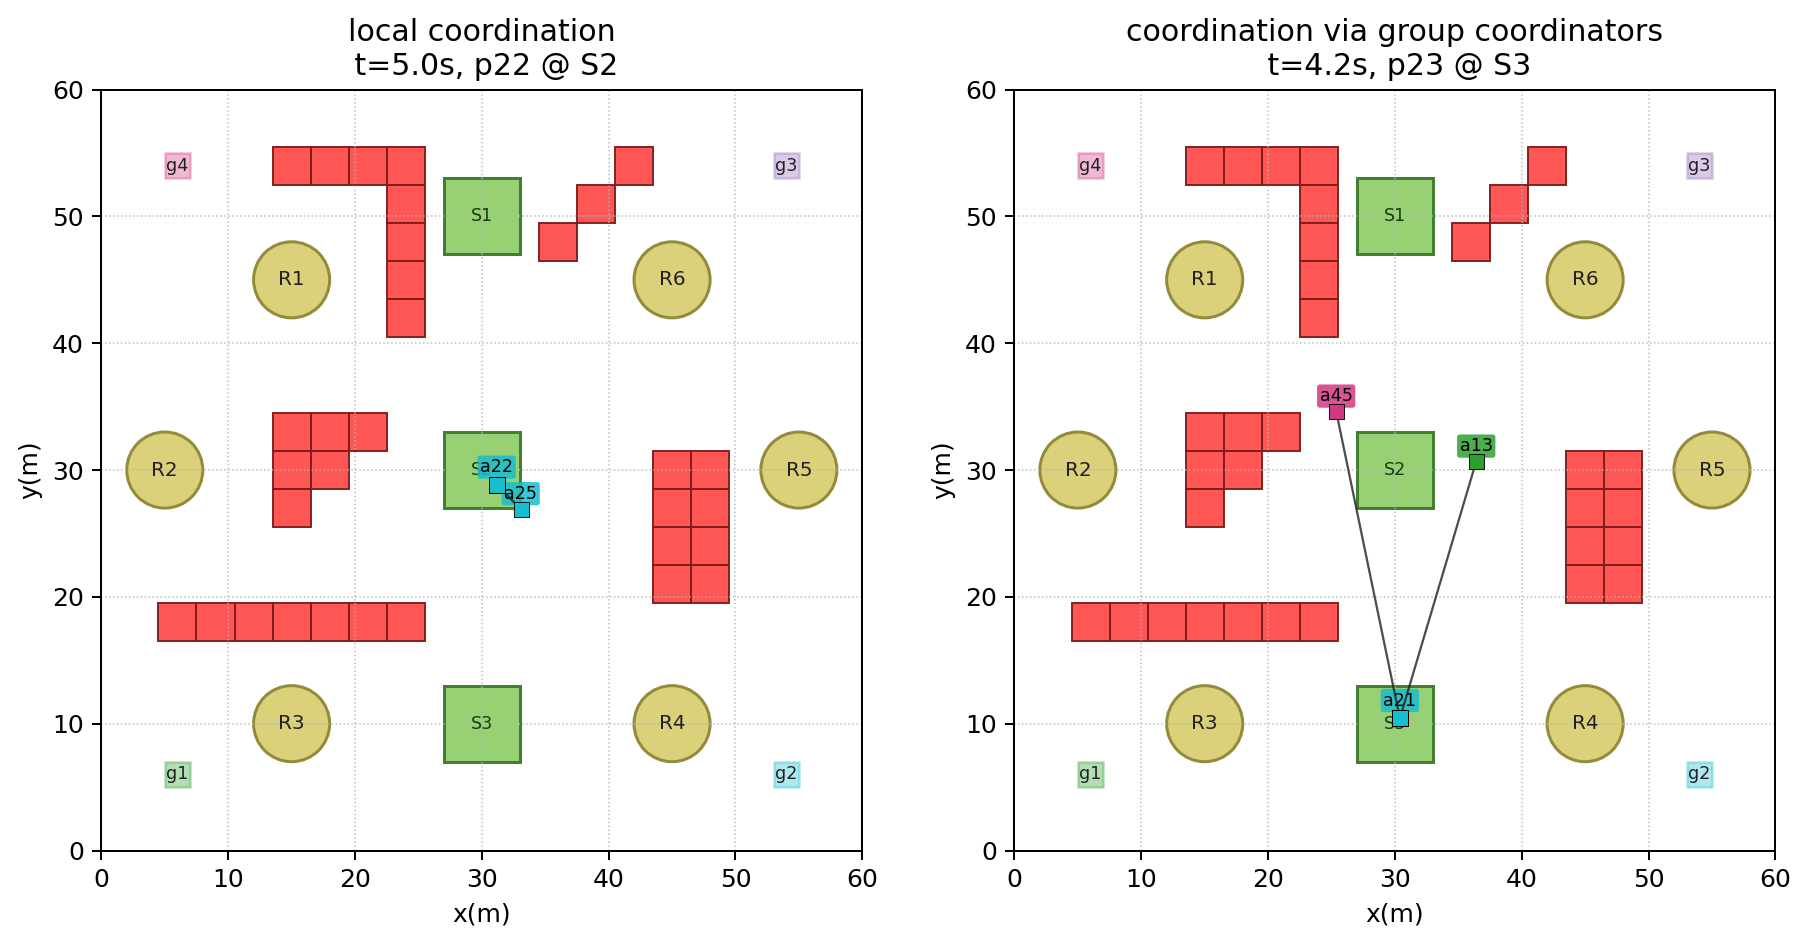
\includegraphics[width=0.9\linewidth]{figures/ch03/ch03_case_two_layer_snapshots.png}
\caption{
Representative coordination events during execution. The left panel shows a
collaborative request resolved through direct local coordination, while the
right panel shows a nonlocal coordination event whose information is routed
through group coordinators. Different colors denote different groups, and
straight segments indicate active communication links during the corresponding
request event.
}
\label{ch03:fig:case_two_layer}
\end{figure}

%==============================
\subsection{Execution results and communication statistics}
\label{ch03:subsec:case_results}

All $20$ robots complete their assigned local tasks by
$t_f=156.2\,\mathrm{s}$. Over the full run, the simulator records
$N_{\mathrm{req}}=46$ coordination-request events. Among them, $15$ requests
are resolved through direct local-neighbor interaction and $31$ require
coordinator-mediated propagation. Hence approximately $32.6\%$ of all requests
are handled locally, whereas the remaining $67.4\%$ require broader
coordination. The run contains $40$ local actions, $46$ collaborative actions,
and $64$ assisting actions, for a total of $150$ executed actions. Thus the
average number of executed actions is $7.5$ per robot, and the overall
execution rate is approximately $150/156.2 \approx 0.96$ actions per second.
Moreover, the ratio $64/46 \approx 1.39$ indicates that a collaborative action
requires more than one assisting action on average, which is consistent with the
action-level dependency relation introduced through $\texttt{Depd}_i$ in
Section~\ref{ch03:sec:collaborative}.
Figure~\ref{ch03:fig:case_execution_snapshots} shows three representative
execution snapshots at $t=31.2\,\mathrm{s}$, $t=93.7\,\mathrm{s}$, and
$t=156.2\,\mathrm{s}$. The faded curves indicate the trajectories already
traveled by the robots. The snapshots show a progressive transition from early
deployment near the base locations, to the dense middle stage in which multiple
collaborative dependencies are active simultaneously, and finally to the
completion stage at which all local tasks have been satisfied. In particular,
the intermediate snapshot at $t=93.7\,\mathrm{s}$ shows several concurrent
dependencies across multiple regions, which demonstrates that the scheme does
not rely on a single global synchronization point. Instead, collaborations are
formed, confirmed, executed, and removed asynchronously according to the local
progress of the involved robots.

\begin{figure}[t!]
\centering
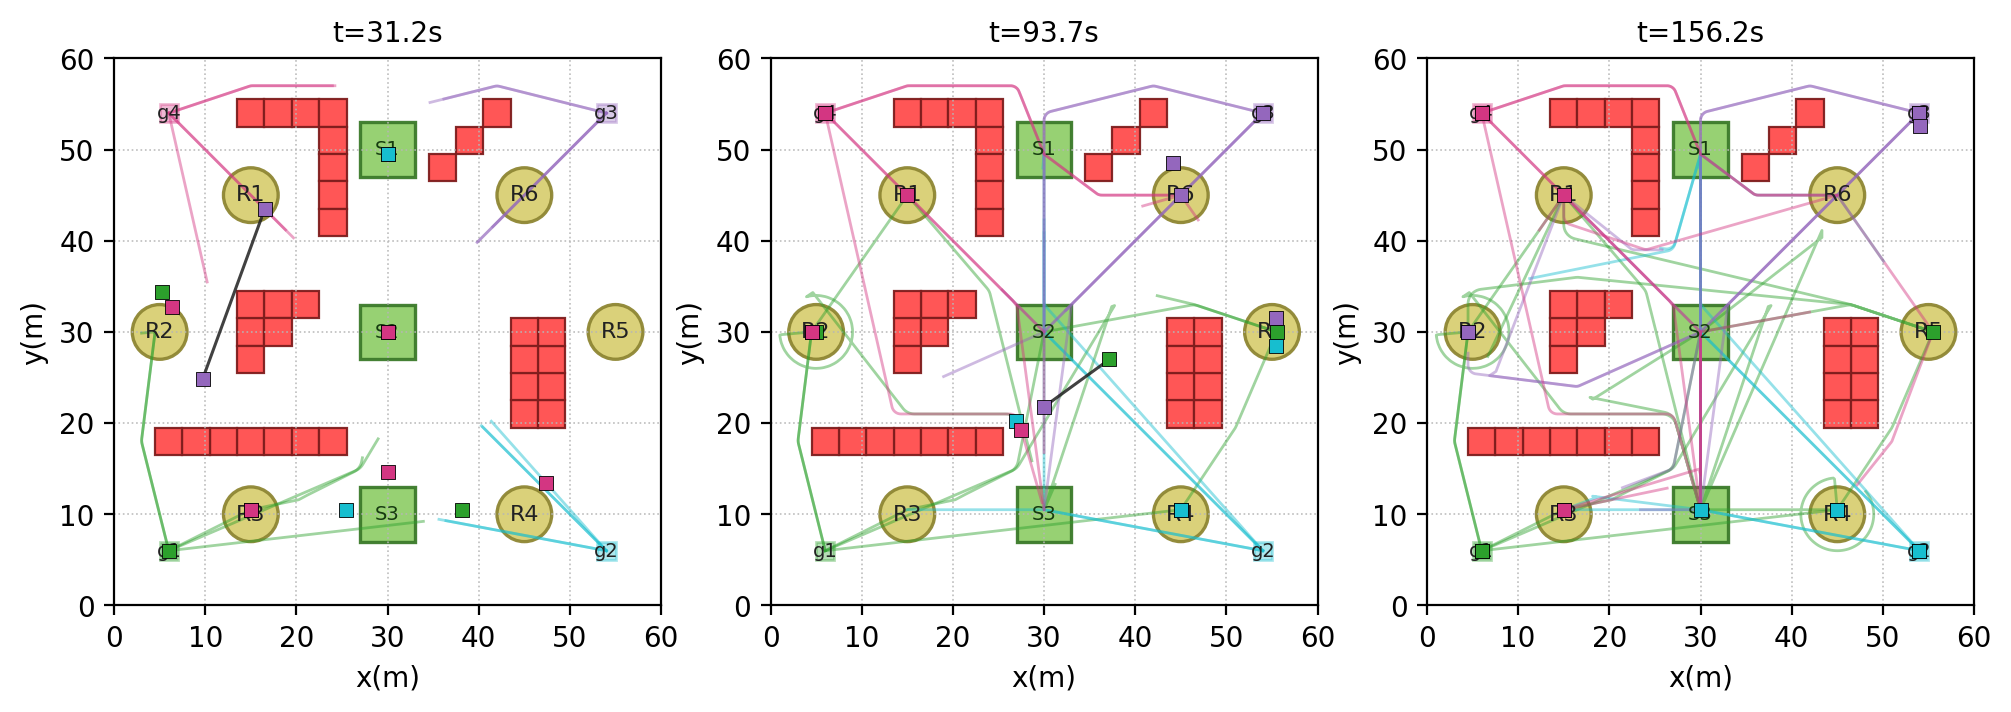
\includegraphics[width=0.9\linewidth]{figures/ch03/ch03_case_execution_snapshots.png}
\caption{
Representative multi-time snapshots of the full execution at
$t=31.2\,\mathrm{s}$, $t=93.7\,\mathrm{s}$, and $t=156.2\,\mathrm{s}$. The
faded curves indicate the trajectories traveled by the robots up to each time
instant. The snapshots visualize how local tasks, assisting tasks, and
collaborative actions become coupled during the execution.
}
\label{ch03:fig:case_execution_snapshots}
\end{figure}

A more detailed view of the asynchronous execution structure is given in
Figure~\ref{ch03:fig:case_actions_timeline}. The horizontal axis denotes time,
and the vertical axis denotes the robot index used in the simulator log. The
labels \texttt{p}, \texttt{d}, \texttt{record}, and \texttt{circle}
denote pick, drop, record, and circle actions; labels prefixed by
\texttt{help\_} denote assisting actions executed in support of a
collaborative action. The timeline shows that collaborative actions are not
inserted by a centralized global schedule. Instead, they are requested when a
collaborative action enters the finite planning horizon and are executed at the
corresponding plan state together with the confirmed assisting actions. This
pattern is consistent with the
finite-horizon request mechanism of Algorithm~\ref{ch03:alg:request} and the
delayed adaptation procedure of Algorithm~\ref{ch03:alg:delay}: only the
affected plan segments are revised, while unrelated robots continue to progress
on their own local tasks.

\begin{figure}[t!]
\centering
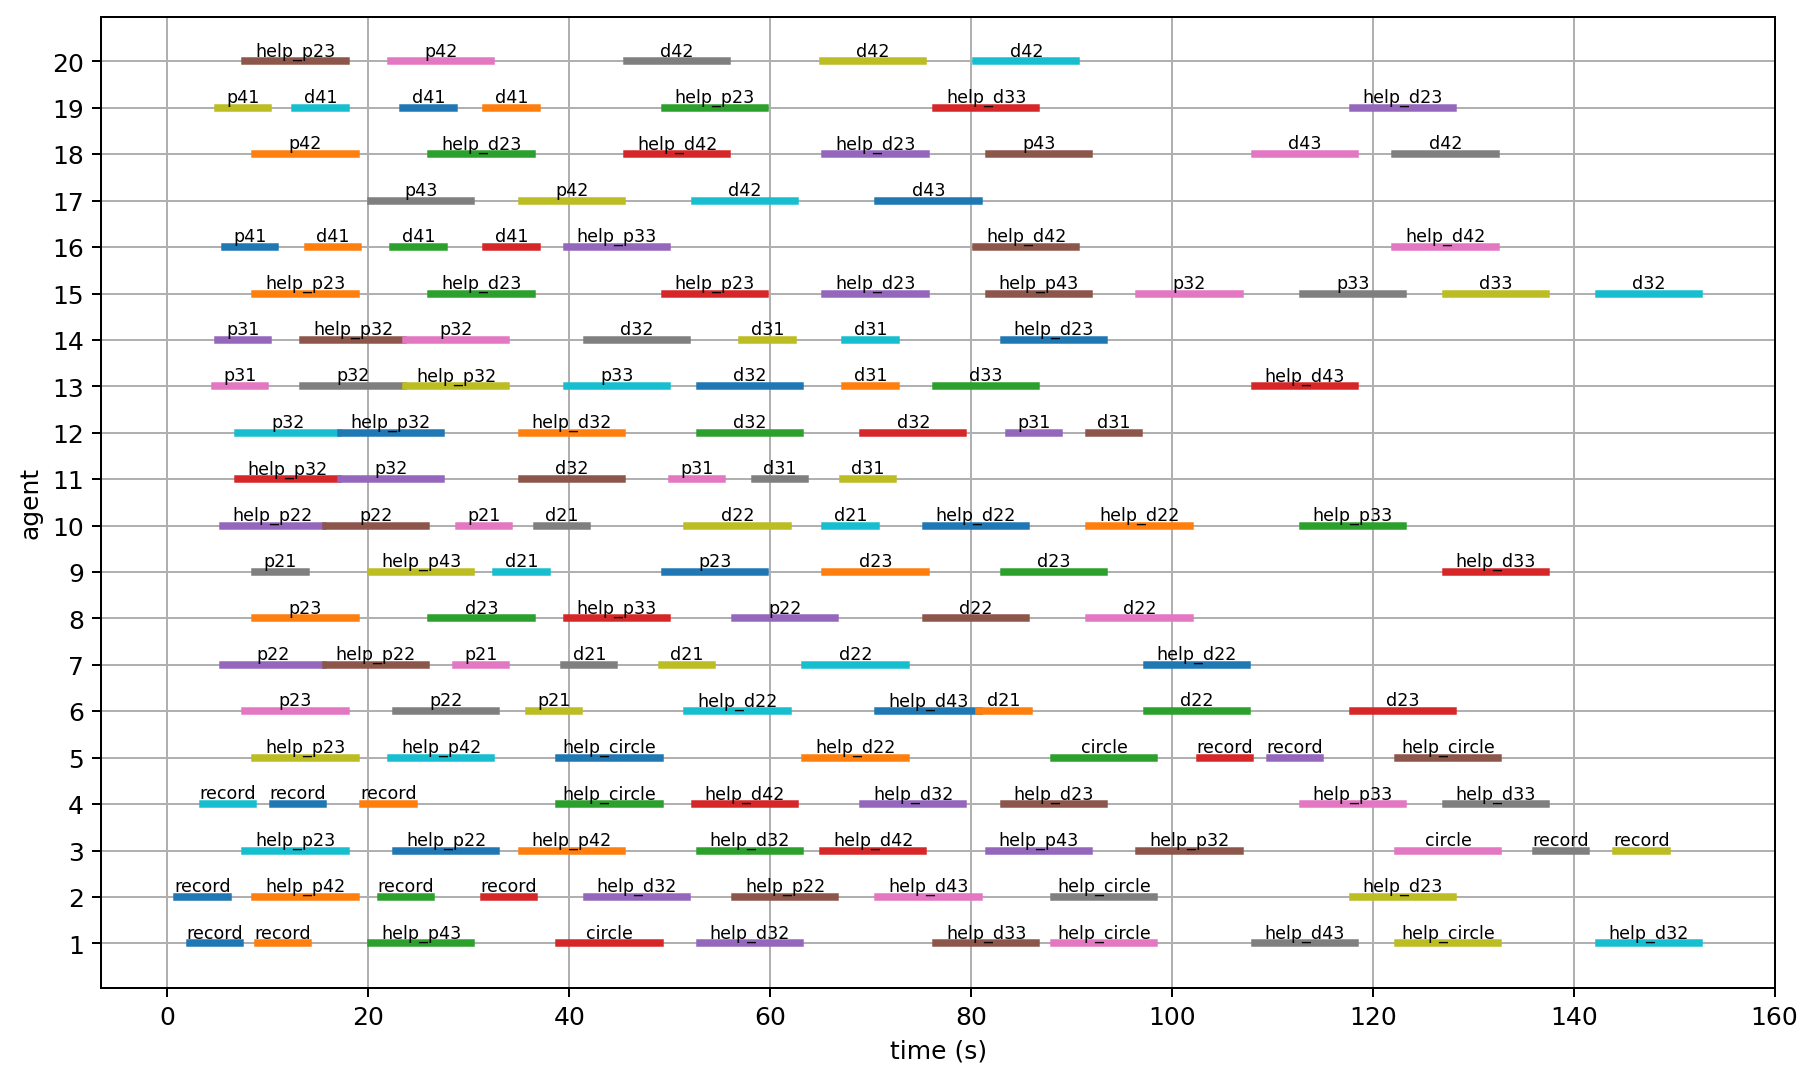
\includegraphics[width=0.9\linewidth]{figures/ch03/ch03_case_actions_timeline.png}
\caption{
Action timeline of all robots during the simulation. The vertical axis shows
the robot index used in the simulator log, and the horizontal axis shows time.
The labels \texttt{p}, \texttt{d}, \texttt{record}, and \texttt{circle}
stand for pick, drop, record, and circle actions, whereas labels prefixed by
\texttt{help\_} denote assisting actions for collaborative tasks.
}
\label{ch03:fig:case_actions_timeline}
\end{figure}

The communication statistics further support this interpretation.
Figure~\ref{ch03:fig:case_messages_over_time} reports the number of messages
exchanged over time. The total number of exchanged messages is
$N_{\mathrm{msg}}=782$, of which $714$ belong to the coordinator-mediated route
and $68$ belong to the direct local-neighbor route. Hence the local route
accounts for only about $8.7\%$ of all messages even though it resolves
$32.6\%$ of all requests. Conversely, coordinator-mediated communication
accounts for about $91.3\%$ of the messages and $67.4\%$ of the requests.
Normalized by the number of requests, the average communication load is about
$17.0$ messages per request, including approximately $23.0$ messages for each
coordinator-mediated request and $4.5$ messages for each local request. The mean
message rate over the full run is approximately
$782/156.2 \approx 5.01$ messages per second. These numbers show that local
coordination is relatively cheap when it is available, while broader
coordination remains event-driven rather than persistent. The message bursts
therefore occur primarily near the instants at which collaborative dependencies
are requested, evaluated, and confirmed, which is precisely the behavior
intended by the distributed online coordination scheme.

\begin{figure}[t!]
\centering
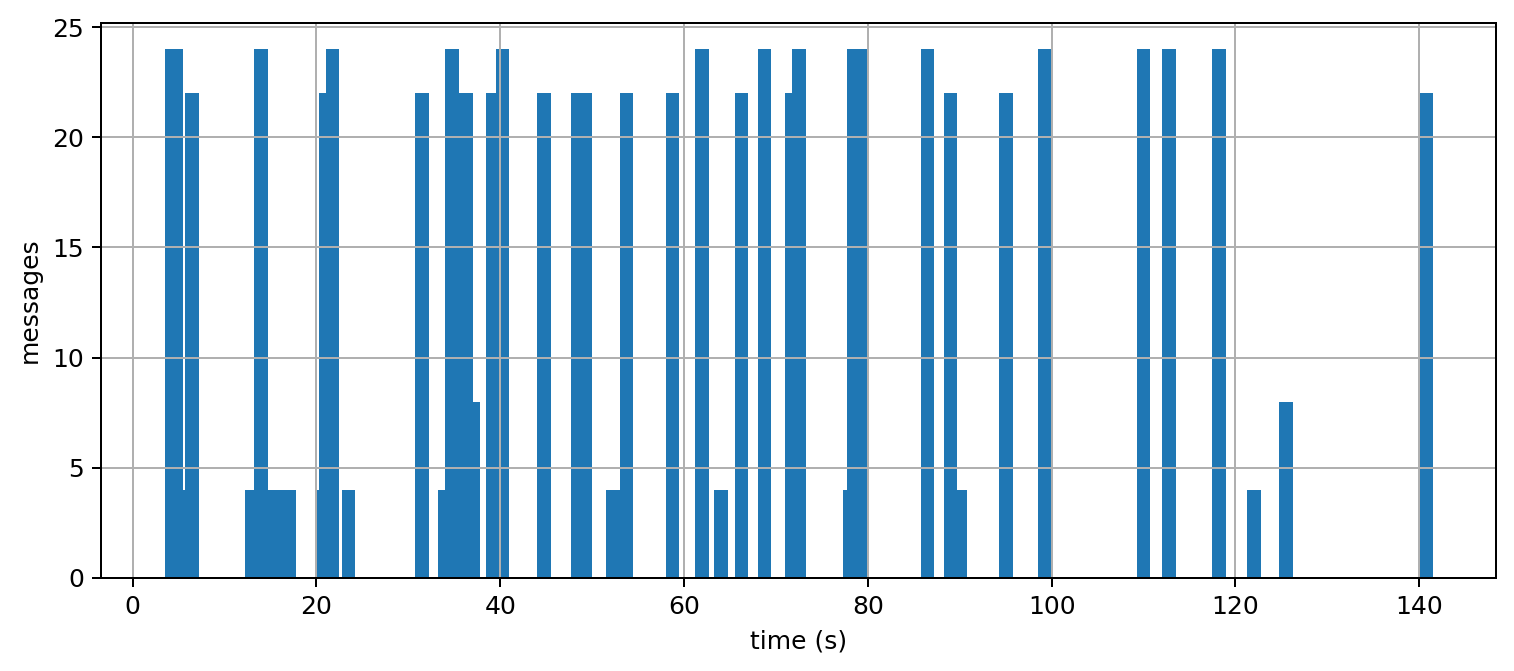
\includegraphics[width=0.9\linewidth]{figures/ch03/ch03_case_messages_over_time.png}
\caption{
Number of exchanged messages over time during the simulation. The communication
load is concentrated near request, reply, confirmation, and adaptation events,
which shows the event-driven nature of the proposed coordination mechanism.
}
\label{ch03:fig:case_messages_over_time}
\end{figure}


Algorithmically, the instance also illustrates why the bottom-up construction is
used instead of composing the full team model. This comparison follows the
complexity estimates reported for the source benchmark of \citet{guo2016task},
and is independent of the reproduced completion time. The centralized product
for the same benchmark class would combine $20$ motion abstractions and the task
automata of all robots; using the reported UAV and UGV automaton sizes, this
would lead to approximately $1600^{20}\cdot 8^5\cdot 46^{15}
\approx 3.5\times 10^{93}$ product states. The distributed implementation
constructs products only at the single-robot level, where typical local product
automata are on the order of $10^5$ states and the reference implementation
synthesizes a local initial policy in about $2\,\mathrm{s}$ on average. Online
coordination is then restricted to the requesting action: the assignment problem
has $|\mathcal{N}_i|\,|\texttt{Depd}_i(\sigma_m)|$ binary variables for a local
request, and only the affected plan segment is delayed or revised when the
request cannot be confirmed. This explains the event-driven message bursts in
Figure~\ref{ch03:fig:case_messages_over_time}: the expensive global product is
avoided, and coordination is achieved  when a collaborative action enters
the finite planning horizon of individual robots.


%==============================
\section{Summary}
\label{sec:ch03_summary}

\rev{This chapter developed multi-robot coordination under prescribed local
temporal tasks.}
\rev{Section~\ref{ch03:sec:task_relaxation_adaptation} combined the local
sensing and plan revision routine of Section~\ref{ch03:sec:partial} with
task-relevant information exchange between robots.}
Section~\ref{ch03:sec:dep-local-collab} then introduced dependent local
tasks with collaborative actions and a distributed execution-time
coordination mechanism for request, reply, assignment, and adaptation.
These developments show how correctness can be
maintained without a monolithic global mission, by coordinating locally
specified tasks whose interactions arise during execution.

